\documentclass[11pt,a4paper,uplatex,dvipdfmx]{ujarticle} 		% for uplatex
%\documentclass[11pt,a4j,dvipdfmx]{jarticle} 					% for platex
%=======================================
% form00_header.tex
%	General header for kakenhiLaTeX,  Moved over from form00_2010_header.tex.
%	2009-09-06 Taku Yamanaka (Osaka Univ.)
%==== General Version History ======================================
% 2006-05-30 Taku Yamanaka (Physics Dept., Osaka Univ.)
% 2006-06-02 V1.0
% 2006-06-14 V1.1 Use automatic calculation for cost tables.
% 2006-06-18 V1.2 Split user's contents and the format.
% 2006-06-20 V1.3 Reorganized user and format files
% 2006-06-25 V1.4 Readjusted all the table column widths with p{...}.
%				With \KLTabR and \KLTabRNum, now the items can be right-justified
%				in the cell defined by p{...}.
% 2006-06-26 V1.5 Use \newlength and \setlength, instead of \newcommand, to define positions.
% 2006-08-19 V1.6 Remade it for 2007 JFY version.
% 2006-09-05 V1.7 Added font declarations suggested by Hoshino@Meisei Univ.
% 2006-09-06 V1.8 Introduced usePDFform flag to switch the form file format.
% 2006-09-09 V1.9 Changed p.7, to allow different heights between years. (Thanks to Ytow.)
% 2006-09-11 V2.0 Added an option to show budget summary.
% 2006-09-13 V2.1 Added an option to show the group.
% 2006-09-14 V2.1.1 Cleaned up Kenkyush Chosho.
% 2006-09-21 V2.2 Generated under a new automatic development system.

% 2007-03-24 V3.0 Switched to a method using "picture" environment.

% 2007-08-14 V3.1 Switched to kakenhi3.sty.
% 2007-09-17 V3.2 Added \KLMaxYearCount
% 2008-03-08 V3.3 Remade it for 2009 JFY version\
% 2008-09-08 V3.4 Added \KLXf ... \KLXh.
% 2011-10-20 V5.0 Use kakenhi5.sty, to utilize array package in tabular environment.
% 2012-08-14 v5.1 Moved preamble and kakenhi5 into the current directory, instead of the parent directory.
% 2012-11-10 v6.0 Switched to kakenhi6.sty.
% 2015-08-26 v6.1 Added KLFirstPageIsLongPage flag.
% 2017-05-27 v7.0 Simplified for the new format.
% 2022-10-27 v7.1 Removed [dvipdfmx] from \usepackage{graphicx}.
%=======================================
% Dummy section and subsection commands.
% With these, some editors (such as TeXShop, etc.) can jump to the (sub)sections.
\newcommand{\dummy}{dummy}% 
\renewcommand{\section}[1]{\renewcommand{\dummy}{#1}}

\usepackage{calc}
\usepackage{geometry}                % See geometry.pdf to learn the layout options. There are lots.
\usepackage{graphicx}
\usepackage{color}
\usepackage{ifthen}
\usepackage{udline}
\usepackage{array}
\usepackage{longtable}
\usepackage{fancyhdr}
 % pieces
%==================================================
% kakenhi7.sty
%==================================================
% v1
% Minimum amount of macros for writing Kakenhi forms.
%
% 2005-10-24 Taku Yamanaka, Physics Dept. Osaka Univ.
%		taku@hep.sci.osaka-u.ac.jp
% 		Macros such as XYBC, etc. were imported from Kakenhi Macro at
% 		http://www.yukawa.kyoto-u.ac.jp/contents/researcher/kakenhi.html .
% 2006-06-04 Taku
%		Added macros to draw boxes if \DrawBox is in the source.
%		This is useful when designing the LaTeX forms.
% 2006-06-14 Taku
%		Added LaTeX macros to add costs 
%		(\KLResetGrandSum, \KLCostItem, \KLSum, \KLGrandSum).
%		Added a macro \Number to supply commas every 3 digits (imported from kkh.mac).
% 2006-06-25 Taku
%		Added \KLTabC, \KLTabR, \KLTabRNum to specify alignments in tables.
%		Please note that \phantom{...} is required for the column, 
%		or otherwise somehow p{...mm} is ignored.
% 2006-08-13 Taku
%		Added \KLItemNumUnitCost . This requires calc.sty.
% 2006-09-06 Taku
%		Added KLGrandTotalValue to add ALL the costs.
%		Also added \KLPrintGrandTotal to print the total on the console.
% 2006-09-09 Taku
%		Added macros to handle "efforts".
% 2006-09-10 Taku
%		Added \KLnewcounter to make series of counters.
%		Modified \KLResetGrandSum and \KLSum to add the sum for 
%		each category and year.
% 2006-09-11 Taku
%		Added \NumC to display LaTeX counter with commas.
% 2006-09-12 Taku
%		Added simple macros to make group table.
% 2006-09-23 Taku
%		Added the 'Fair License' notification.
% 2006-10-22 Taku
%		Initialize KLNumPeople to -1, so that the first header row will not be included in the count.
%====================================================
% v2
% 2007-03-24 Taku
%		Instead of using Kakenhi Macros to position items, 
%		switched to a new method using
%		"picture" environment.  The origin of the coordinate is set to 
%		the lower left corner of the paper.  The positions are given in "points", 
%		as can be read by gv. These methods were suggested by 
%		Tsutomu Sakurai at Saitama Univ..
% 2007-03-30 Taku
%		The sum of each category and year is made using 
%		macros \KLItemCost, etc., instead of \KLSum.  This is a step toward
%		automatically aligning category sums in the same year, in some forms.
% 2007-04-02 Taku
%		Added \KLBudgetMiniTabular, \KLMiniSum, etc. to handle
%		budget tables with multiple category columns.
% 2007-05-04 Taku
%		Added \multicolumnDottedLine .
%==================================================
% v3 
% 2007-08-14 Taku
%		Simplified page handling, by introducing \KLBeginSinglePage,
%		\KLPageRange, etc..
% 2007-09-01 Taku
%		Added a new command, \KLItemNumUnitCostLocation , 
%		and \KLAddCost to clean things up.
% 2007-09-06 Taku
%		Set \KLEven/OddLeft/RightEdge parameters in \KLWaterMark.
%		Without it, if \KLLeftEdge or \KLRightEdge is used inside watermark,
%		it generated a very obscure error message, which was hard to track down.
% 2007-09-09 Taku
%		Removed clearring \thiswatermark in \KLClearWaterMarks.
% 2007-09-12 Taku
%		Added \KLPriorityItemNumUnitCostTwo for Tokusui.
% 2007-09-14 Taku
%		Added \KLItemNumUnitCostTwo for tokutei_koubo.
% 2007-09-17 Taku
%		In \KLAddCost, costs are added only if it is within the defined year range.
% 2008-09-02 Taku
%		  Added \KLMonthPriorityItemNumUnitCostTwo for tokutei_keizoku.
% 2008-09-07 Taku
%		   Use \KLJFY to print year in budget tables.
% 2008-10-21 Taku
%			Added KLItemNumUnitCostInParen for shorei.
% 2009-09-03 Taku
%			Added \dottedLine .
%==================================================
% v4
% 2009-09-06 Taku
%			Added macros for partial typesetting.
% 2009-09-12 Taku
%			Added macros for showing coordinates and edges.
% 2009-09-13 Taku
%			Added macros to show boxes and minipage frames and their corner coordinates.
% 2010-03-04 Taku
%			Moved macros for calculating lengths and positions from form07_header.tex to here.
% 2010-04-11 Taku
%			Added \KLItemCostOne for jisedai, and necessary flags to print budget sums before 
%			the detailed budget table.
%==================================================
% v5
% 2011-10-20 Taku
%			By using array package within tabular environment, the following macros were simplified:
%			\KLTabC, \KLTabR, \KLBudgetMiniTabular, 
%			New Macros:
%			\KLCC, \KLCR
% 2011-10-24 Taku
%			Removed using \KLTabR from most of the budget tables.
% 2011-10-26 Taku
%			Added KLMyBudget.
%			Modified KLYearItemNumUnitCostTwo to just put the JFY if the second item is blank.  (For Kiban S)
% 2012-03-10 Taku
%			Changed the tabcolsep for \KLMyBudget to 0pt.
% 2012-08-14 Taku
%			Moved xxx_forms_pdf and _eps directories to under mother.
% 2012-09-09	Taku
%			Added \KLbibitem(B) and \KLcite(B).
% 2012-09-16	Taku
%			Added \KLOtherApplication, \KLOtherApplicationReasons, and \KLOtherFundReasons
%			for tokusui (and maybe for others in the future).
%==================================================
% v6
% 2012-11-10	Taku
% 			Modified \KLOtherApplicationReasons and \KLOtherFundReasons to make the tables compact.
%			These were in hook3.tex for the 2013 version.
%			Added \KLOtherApplicationDiff for many shumokus.
%			Removed \KLbibitemB and \KLciteB.
%			Changed \KLbibitem to use a dedicated column for numbering.
% 2012-11-11	Taku
%			Added \KLItemSetCostLocationInfo and \KLItemCostInfo.
% 2013-09-19	Taku
%			Added \KLOtherPD and \KLOtherPDShort to enter JSPS PD for other funds.
% 2013-10-02	Taku
%			Changed \KLbibItem, not to use a dedicated column for numbering, 
%			because otherwise the label defined in \label{...} cannot be used in @currentlabel.
% 2014-09-22	Taku
%			Added \KLCL for filling narrow tabular cells in English.  
%			(Suggested by Frank Bennett.)
% 2014-11-08	Taku
%			Added an instruction in \KLCheckPageLimit.
% 2015-08-23	Taku
%			Added NumCk to show numbers divided by 1000 (truncated).
% 2015-08-24	Taku
%			Introduced \KLLongPage and \KLSimpleLongPage to offer floating environment in 
%			single-page-frames.
%=====================================================
% v7
%	Frames are gone!  Simplify kakenhiLaTeX to benefit from 
%	the new style.
% 2017-05-03	Taku
%			Added \KLAnotherFund .
% 2017-05-27	Taku
%			Made \KLBeginSubject and \KLEndSubject to handle new 
%			mother file style.
% 2017-08-17 Taku
%	Added \KLItemCostNoYear and \KLEndBudgetNoYear for kokusai_kyoudou.
% 2017-08-19	Taku
%			Updated \KLBeginSubject and \KLEndSubject to handle 
%			various headers.
% 2017-08-20	Taku
%			\KLBeginSubject calls \KLFirstPageStyle and \KLDefaultPageStyle
%			which should be defined for each shumoku (or JSPS/MEXT).
%			This is to pass the subject name etc. to the header.
% 2017-08-27	Taku
%			Set section number in \KLBeginSubject.
% 2017-08-29	Taku
%			Moved over KLShumokuFirstPageStyle and KLShumokuDefaultPageStyle.
%			Added jsps-abs-p1-header, jps-abs-subject-header, and 
%			jsps-abs-default-header as arguments to \KLShumoku***Header.
% 2017-09-02	Taku
%			Added \KLBeginSubjectWithHeaderCommands for more flexible header style.
% 2017-09-03	Taku
%			Added \vspace*{-4mm} after \includegraphics in \KLBeginSubject*.
% 2017-09-05	Taku
%			Removed now-the-old commands.
% 2020-01-02	Taku
%			Added more numbers to \KLJint for gakuhen_a.
% 2020-01-15	Taku
%			Changed the horizontal position (none --> -3mm) 
%			and the width of the top boxes for headers (\linewidth --> 1.02\linewidth)
%			to reproduce the original boxes.  
%			This became necessary because the margins were set correctly in form02_header.tex.
% 2021-01-29	Taku
%			Set section counter and reset subsection counter only if the section # is given for
%			\KLBeginSubject and \KLBeginSubjectWithHeaderCommands .
% 2022-01-26	Taku
%			Changed the scale for the top boxes from 1.03 to 1.01, 
%			and \hspace from -3mm to -2mm.  (DC)
% 2022-02-23	Taku
%			Introduced \KLBoxOffset and \KLBoxScale for flexibility.
% 2022-03-20	Taku
%			Added '%' after \hspace{ } before incldegraphics.
% 2022-08-03	Taku
%			Use width=\KLBoxWidth, instead of \KLBoxScale*\linewidth which depents on
%			\linewidth.  (I should have noticed it earlier.)
% 2023-03-09	Taku
%			Added \vspace*{\KLBoxVOffset} to \KLBeginSubject.
% 2023-07-10	Taku
%			Added \includegraphics_full_width to place full-width 
%			instruction box images.
%			This is used also for \KLBeginSubject and 
%			\KLBeginSubjectWithHeaderCommands.  
%			\KLBoxOffset and \KLBoxWidth are not needed anymore.
%			Why didn't I think of it (-1in-\oddsidemargin) before??
% 2023-07-18	Taku
%			Old LaTeX cannot handle \hspace{-1in-\oddsidemargin}.
%			Changed to calculate the length by \setlength, and then use the result in \hspace.
%=====================================================

%=====================================================
% Macro to supply commas every 3 digits (up to 9 digits)
%	Imported from kkh.mac for Kakenhi Macro.
%=====================================================
%
\newif\ifNumWithCommas \NumWithCommastrue
\def\NumWithCommas{\NumWithCommastrue}
\def\NumWithoutCommas{\NumWithCommasfalse}
\newcount\Numa
\newcount\Numb
\def\Numempty{}%output blank if "-0" is given
\def\Number#1{\edef\Numpar{#1}\ifx\Numempty\Numpar\else%
\ifNumWithCommas\Numa=#1\relax
\ifnum\Numa>999999\divide\Numa by 1000000
\number\Numa,%
\multiply\Numa by -1000000\advance\Numa by #1\relax
\Numb=\Numa\divide\Numa by 1000
\ifnum\Numa<100 \ifnum\Numa<10 0\fi0\fi\number\Numa,%
\multiply\Numa by -1000\advance\Numa by \Numb
\ifnum\Numa<100 \ifnum\Numa<10 0\fi0\fi\number\Numa%
\else\ifnum\Numa>999\divide\Numa by 1000
\number\Numa,%
\multiply\Numa by -1000\advance\Numa by #1\relax
\ifnum\Numa<100 \ifnum\Numa<10 0\fi0\fi\number\Numa%
\else\number\Numa\fi\fi\else\number#1\fi\fi}

%======================================================
% Macro to display LaTeX counter with commas every 3 digits.
%======================================================
\newcommand{\NumC}[1]{\Number{\value{#1}}}

\newcounter{kyen}
\newcommand{\NumCk}[1]{%
	\setcounter{kyen}{\arabic{#1}/1000}
	\Number{\value{kyen}}
}

%======================================================
% Macros to align (right-justify, center) elements within a tabular cell
% whose width is defined by p{...}.
% 2006-06-25 Taku
% 	These are necessary, because the cell width should be given explicitly
% 	by p{...mm} to match the given table in a tabular environment.  
% 	One could allocate a width with \phantom{...},
% 	but it is a little tricky, since it depends on the font size.
%======================================================

%---------------------------------------------------------------------
% Center text within a tabular cell allocated by p{...}
%\newcommand{\KLTabC}[1]{\multicolumn{1}{c}{#1}}
\newcommand{\KLTabC}[1]{\centering\arraybackslash#1}
% This new method does not require a dummy table row to put them in correct columns.
%
% This should be used in tabular definition, as:
%	\begin{tabular}[t]{>{\KLCC}p{30pt}p{50pt}}
\newcommand{\KLCC}{\centering\arraybackslash}

%---------------------------------------------------------------------
% Right justify text within a tabular cell allocated  by p{...}
%\newcommand{\KLTabR}[1]{\multicolumn{1}{r@{\ }}{#1}}
\newcommand{\KLTabR}[1]{\raggedleft\arraybackslash#1}

% This should be used in tabular definition, as:
%	\begin{tabular}[t]{>{\KLCR}p{30pt}p{50pt}}
\newcommand{\KLCR}{\raggedleft\arraybackslash}%

%---------------------------------------------------------------------
% Right justify number (with comma every 3 digits) 
% within a tabular cell allocated by p{...}
\newcommand{\KLTabRNum}[1]{\KLTabR{\Number{#1}}}

%---------------------------------------------------------------------
% Left justify text within a tabular cell allocated by p{...}
% This should be used in tabular definition, as:
%	\begin{tabular}[t]{>{\KLCL}p{30pt}p{50pt}}
\newcommand{\KLCL}{\raggedright\arraybackslash}%

%=================================================
%  counter tools
%=================================================
\newcounter{KLtmp}

%------------------------------------------------------------------------------
% Makes a set of counters, with prefix #1, followed by 
% suffix ranging from 0 to #2 - 1.
% For example, \KLnewcounter{mine}{3} makes counters
% mine0, mine1, and mine2 .
%-------------------------------------------------------------------------------
\newcommand{\KLnewcounter}[2]{
	\setcounter{KLtmp}{0}
	
	\whiledo{\value{KLtmp} < #2}{
		\newcounter{#1\arabic{KLtmp}}
		\stepcounter{KLtmp}
	}
}

%------------------------------------------------------------------------------
% Dumps the contents of the counters.
%------------------------------------------------------------------------------
\newcommand{\KLdumpcounter}[2]{
	\setcounter{KLtmp}{0}
	
	\whiledo{\value{KLtmp} < #2}{
		#1\arabic{KLtmp} : \arabic{#1\arabic{KLtmp}}\\
		\stepcounter{KLtmp}
	}
}

%=======================================================
% LaTeX macros to add costs.
%	2006-06-14 Taku Yamanaka
%=======================================================
\newcounter{KLCost}				% to calculate cost = #units x unit cost
\newcounter{KLGrandTotalValue}		% for the grand total of all the categories in all years
\setcounter{KLGrandTotalValue}{0}

\newcommand{\KLCostCategory}{KLequipments}
\newcounter{KLYearCount}
\newcounter{KLPrintYear}

% Make counters for annual sums for each category-----------------------
\newcommand{\KLMaxYear}{8}
\KLnewcounter{KLequipments}{\KLMaxYear}
\KLnewcounter{KLexpendables}{\KLMaxYear}
\KLnewcounter{KLdomestic}{\KLMaxYear}
\KLnewcounter{KLforeign}{\KLMaxYear}
\KLnewcounter{KLtravel}{\KLMaxYear}
\KLnewcounter{KLgratitude}{\KLMaxYear}
\KLnewcounter{KLmisc}{\KLMaxYear}
\KLnewcounter{KLAnnualSum}{\KLMaxYear}

%------------------------------------------------
% Add up the given cost to category-year sum, category sum, year-sum, and total.
% 2007-09-01 Taku
% 2007-09-17 Taku: Add costs only if it is within the defined year range.
%------------------------------------------------
\newcommand{\KLAddCost}[1]{%
	\ifthenelse{\value{KLYearCount} > \value{KLMaxYearCount}}{%
		%pass
	}{%
		\addtocounter{\KLCostCategory0}{#1}%
		\addtocounter{\KLCostCategory\arabic{KLYearCount}}{#1}%
		\addtocounter{KLAnnualSum\arabic{KLYearCount}}{#1}%
		\addtocounter{KLAnnualSum0}{#1}%
		\ifthenelse{\equal{\KLCostCategory}{KLdomestic}}{%
			\addtocounter{KLtravel0}{#1}%
			\addtocounter{KLtravel\arabic{KLYearCount}}{#1}%
		}{}%
		\ifthenelse{\equal{\KLCostCategory}{KLforeign}}{%
			\addtocounter{KLtravel0}{#1}%
			\addtocounter{KLtravel\arabic{KLYearCount}}{#1}%
		}{}%
	}%
}


\newcommand{\KLClearWaterMarks}{%
	%--empty watermarks
	\watermark{}
%	\thiswatermark{}
	\rightwatermark{}
	\leftwatermark{}
}

\newcommand{\KLInput}[1]{%	The macros defined inside the file are only valid within the file.
	\begingroup
	\input{#1}
	\endgroup
}

%================================
% For 2017 new style without frames
%================================
\newcommand{\KLShumokuFirstPageStyle}[5]{%
%	Defines the header for the first page.
%	Called from \KLBeginSubject.
%--------------------------------
%	#1: page style name
%	#2: 様式
%	#3: 研究種目名
%	#4: 項目名
%	#5: sectionNo
%--------------------------------
	\ifthenelse{\equal{#1}{jsps-p1-header}}{%
		\JSPSVeryFirstPageStyle{#1}{#2}{#3}{#4}{#5}
	}{%
		\ifthenelse{\equal{#1}{jsps-abs-p1-header}}{%
			\JSPSVeryFirstPageStyle{#1}{#2}{#3 概要}{#4}{#5}
		}{%
            		\ifthenelse{\equal{#1}{jsps-subject-header}}{%
            			\JSPSFirstSubjectPageStyle{#1}{#2}{#3}{#4}{#5}
            		}{%
				\ifthenelse{\equal{#1}{jsps-abs-subject-header}}{%
            				\JSPSFirstSubjectPageStyle{#1}{#2}{#3 概要}{#4}{#5}
				}{%
                    			\thispagestyle{#1}
				}
            		}
		}
	}
}

\newcommand{\KLShumokuDefaultPageStyle}[5]{%
%	Defines the default header.
%	Called from \KLBeginSubject.
%--------------------------------
%	#1: page style name
%	#2: 様式
%	#3: 研究種目名
%	#4: 項目名
%	#5: sectionNo
%--------------------------------
	\ifthenelse{\equal{#1}{jsps-default-header}}{%
		\JSPSDefaultPageStyle{#1}{#2}{#3}{#4}{#5}
	}{%
		\ifthenelse{\equal{#1}{jsps-abs-default-header}}{%
			\JSPSDefaultPageStyle{#1}{#2}{#3 概要}{#4}{#5}
		}{%
            		\pagestyle{#1}
		}
	}
}

\newcommand{\KLSubjectName}{}
\newcommand{\KLSubjectMaxPages}{}
\newcommand{\KLSubjectEndPage}{}
\newcounter{KLSubjectEndPage}
\setcounter{KLSubjectEndPage}{0}

\newcommand{\KLSubjectCheckNPages}{%
%	\arabic{page}, \arabic{KLSubjectEndPage}\\
	\ifthenelse{\value{page}>\value{KLSubjectEndPage}}{
		{\LARGE「\KLSubjectName」は \KLSubjectMaxPages\ ページ以内で書いてください。}
		\clearpage
	}{%
	}
}

\newcommand{\KLSubjectAdvancePages}{%
	\renewcommand{\KLSubjectEndPage}{\value{KLSubjectEndPage}}
	\ifthenelse{\value{page}<\KLSubjectEndPage}{%
		\phantom{x}\clearpage
	}{}
	% Advance page if necessary
	\ifthenelse{\value{page}<\KLSubjectEndPage}{%
		\phantom{x}\clearpage
	}{}
	% Advance page if necessary
	\ifthenelse{\value{page}<\KLSubjectEndPage}{%
		\phantom{x}\clearpage
	}{}
	% Advance page if necessary
	\ifthenelse{\value{page}<\KLSubjectEndPage}{%
		\phantom{x}\clearpage
	}{}
	% Advance page if necessary
	\ifthenelse{\value{page}<\KLSubjectEndPage}{%
		\phantom{x}\clearpage
	}{}
}	

\newcommand{\KLJInt}[1]{%
% Returns full-width numerical character.
	\ifthenelse{\equal{#1}{1}}{1}{%
	\ifthenelse{\equal{#1}{2}}{2}{%
	\ifthenelse{\equal{#1}{3}}{3}{%
	\ifthenelse{\equal{#1}{4}}{4}{%
	\ifthenelse{\equal{#1}{5}}{5}{%
	\ifthenelse{\equal{#1}{6}}{6}{%
	\ifthenelse{\equal{#1}{7}}{7}{%
	\ifthenelse{\equal{#1}{8}}{8}{%
	\ifthenelse{\equal{#1}{9}}{9}{%
	\ifthenelse{\equal{#1}{10}}{10}{%
	\ifthenelse{\equal{#1}{11}}{11}{%
	\ifthenelse{\equal{#1}{12}}{12}{%
	\ifthenelse{\equal{#1}{13}}{13}{%
	\ifthenelse{\equal{#1}{14}}{14}{%
	\ifthenelse{\equal{#1}{15}}{15}{%
	\ifthenelse{\equal{#1}{16}}{16}{%
	\ifthenelse{\equal{#1}{17}}{17}{%
	#1}}}}}}}}}}}}}}}}}%
}

\newlength{\KLFWHOffset}

\newcommand{\includegraphicsFullWidth}[1]{%
	\noindent%
%	\hspace{-1in-\oddsidemargin}%	New LaTeX (2020) can handle this, but old ones (2018) cannot.
	\setlength{\KLFWHOffset}{-1in-\oddsidemargin}%
	\hspace{\KLFWHOffset}%		For old LaTeX
	\includegraphics[width=\paperwidth]{#1}%
}

\newcommand{\KLBeginSubject}[8]{%
%----------------------------------------------------
%	#1: subjectNo
%	#2: sectionNo
%	#3: sectionJ
%	#4: maxPages
%	#5: pageLengthStyle ('V' for variable, 'F' for fixed)
%	#6: pageCounter (set page counter to this value if the argument exists.
%	#7: subjectFirstPageHeader (header for the first page)
%	#8: defaultPageHeader
%----------------------------------------------------
	\ifthenelse{\equal{#2}{}}{%
	}{%
	    	\setcounter{section}{#2}
	    	\setcounter{subsection}{0}
	}
	\setcounter{subsubsection}{0}
	\renewcommand{\KLSubjectName}{#3}
	\renewcommand{\KLSubjectMaxPages}{#4}
	
	\ifthenelse{\equal{#6}{}}{%
	}{%
		\setcounter{page}{#6}
	}
	
	\setcounter{KLSubjectEndPage}{\value{page}}
	\addtocounter{KLSubjectEndPage}{#4}
	
	\ifthenelse{\equal{#7}{}}{%
		% pass
	}{%
		\KLShumokuFirstPageStyle{#7}{\様式}{\研究種目header}{#3}{#2}
	}
	
	\ifthenelse{\equal{#8}{}}{%
		% pass
	}{%
		\KLShumokuDefaultPageStyle{#8}{\様式}{\研究種目header}{#3}{#2}
	}
	
	\vspace*{\KLBoxVOffset}%
%	\noindent
%	\hspace{\KLBoxOffset}%
%	\includegraphics[width=\KLBoxScale\linewidth]{subject_headers/\KLYoshiki_#1.pdf}\\
	\includegraphicsFullWidth{subject_headers/\KLYoshiki_#1.pdf}
	\vspace*{-4mm}
}

\newcommand{\KLNullHeader}[5]{}
% Dummy command for No header.
% This was introduced to avoid error caused in statement \ifthenelse{\equal{#8}{}} .

\newcommand{\KLBeginSubjectWithHeaderCommands}[8]{%
%----------------------------------------------------
%	#1: subjectNo
%	#2: sectionNo
%	#3: sectionJ
%	#4: maxPages
%	#5: pageLengthStyle ('V' for variable, 'F' for fixed)
%	#6: pageCounter (set page counter to this value if the argument exists.
%	#7: LaTeX command for subjectFirstPageHeader (header for the first page)
%	#8: LaTeX command for defaultPageHeader
%----------------------------------------------------
	\ifthenelse{\equal{#2}{}}{%
	}{%
		\setcounter{section}{#2}
		\setcounter{subsection}{0}
	}
	\setcounter{subsubsection}{0}
	\renewcommand{\KLSubjectName}{#3}
	\renewcommand{\KLSubjectMaxPages}{#4}
	
	\ifthenelse{\equal{#6}{}}{%
	}{%
		\setcounter{page}{#6}
	}

	\setcounter{KLSubjectEndPage}{\value{page}}
	\addtocounter{KLSubjectEndPage}{#4}
	
	#7{#7}{\様式}{\研究種目header}{#3}{#2}
	#8{#8}{\様式}{\研究種目header}{#3}{#2}
	
	\vspace*{\KLBoxVOffset}%
%	\noindent
%	\hspace{\KLBoxOffset}%
%	\includegraphics[width=\KLBoxWidth]{subject_headers/\KLYoshiki_#1.pdf}\\
	\includegraphicsFullWidth{subject_headers/\KLYoshiki_#1.pdf}
	\vspace*{-4mm}
}

\newcommand{\KLEndSubject}[1]{%
%	#1: pageLengthStyle ('V' for variable, 'F' for fixed)
		\clearpage % This should be done to update page counter for checking.
		\KLSubjectCheckNPages
		\ifthenelse{\equal{#1}{F}}{%
			\KLSubjectAdvancePages
		}{%
		}
}

%==================================================
% Miscellaneous macros
%==================================================

%----------------------------------------------------------------------
% Draw dotted lines across a multiple column table
%----------------------------------------------------------------------
\newcommand{\multicolumnDottedLine}[1]{%
%	\multicolumn{#1}{@{\hspace{-2mm}}c}{\dotfill}\\%
	\multicolumn{#1}{@{}c}{\dotfill}\\%
}

\newcommand{\dottedLine}{%
	\\\noindent
	\dotfill\\
}

%----------------------------------------------------------------------
% Solid line
%----------------------------------------------------------------------
\newlength{\KLLineLength}
\newcommand{\solidLine}[1]{
%----------- keep an empty line between here and \noindent so that it works after normal text and list.

	\noindent
	\hspace*{-10pt}
	\rule[10pt]{\textwidth}{#1}% #1 = 0.5pt, ....
	\vspace*{-10pt}
}

\newcommand{\KLLine}{%
	\solidLine{1pt}
}

%----------------------------------------------------------------------
% publication list (Thanks to Tetsuo Iwakuma [bulletin board #876])
%----------------------------------------------------------------------
\newcounter{KLBibCounter}

\makeatletter	
	\newcommand{\KLbibitem}{%
		\stepcounter{KLBibCounter}%
		\let \@currentlabel \theKLBibCounter
		\arabic{KLBibCounter}. %
	}
\makeatother

\newcommand{\KLcite}[1]{[\ref{#1}]}

%==================================================
%Fair License

%<Copyright Information>

%Usage of the works is permitted provided that this
%instrument is retained with the works, so that any entity
%that uses the works is notified of this instrument.

%DISCLAIMER: THE WORKS ARE WITHOUT WARRANTY.

%[2004, Fair License: rhid.com/fair]
%==================================================
% You may edit/modify this package at your own risk.
% If there are important fixes or changes that you think should be 
% reflected in the standard distribution, please notify:
%	taku@hep.sci.osaka-u.ac.jp  .
%==================================================
 % pieces
% form01_header.tex
% 2017-05-28 Split from form00_header.tex to move \input{kakenhiLaTeX7.sty} to mother_1.tex.
% 2010-01-15 Adjusted margins.
% 2022-02-23 Introduced \KLBoxOffset and \KLBoxScale.
% 2022-07-25 Introduced \KLBoxVOffset.
% ===== Parameters for KL (Kakenhi LaTeX) ========================
%%\geometry{noheadfoot,scale=1}  %scale=1 resets margins to 0
\setlength{\unitlength}{1pt}

\newlength{\KLCella}
\newlength{\KLCellb}
\newlength{\KLCellc}
\newlength{\KLCelld}
\newlength{\KLCelle}
\newlength{\KLCellf}

\newcounter{KLMaxYearCount}	% # of years for the proposal
\newcommand{\KLCLLang}{}	% language-dependent left-justification in tabular

% ===== format and header =========
% 2020-01-15: Reset it to match the margins (25 mm on sides, 20 mm on top and bottom). 
% A4: 294 mm x 210 mm.  
% LaTeX's default margin is 1 inch = 25.4 mm.
\setlength{\oddsidemargin}{-1pt}	% (25.0 - 25.4) / 25.4 * 72 pt/inch = -1 pt
\setlength{\evensidemargin}{-1pt}
\setlength{\textwidth}{453pt}		% (210 - 25*2) / 25.4 * 72 = 453 pt
\setlength{\topmargin}{-61pt}	% This and \headheight determine the actual top margin
\setlength{\textheight}{254mm}		% (294 - 20*2) = 254 mm

\setlength{\headheight}{48pt}
\setlength{\headsep}{3pt}

\cfoot{}
\renewcommand{\headrulewidth}{0pt}

\newcommand{\KLBoxVOffset}{-12pt}
\newcommand{\KLBoxOffset}{-25mm}
\newcommand{\KLBoxScale}{1.313}
\newcommand{\KLBoxWidth}{210mm}

\pagestyle{empty}
% ==== other applications table =========
\newcommand{\KLTableHeaderFont}{\fontsize{8.2}{11}\selectfont}
\newcommand{\KLTableHeaderSmallFont}{\fontsize{7.5}{10}\selectfont}
\newcommand{\KLTableHeaderSmallerFont}{\fontsize{7}{10}\selectfont}

 % pieces
% ===== Global year-dependent definitions for the Kakenhi form ===========
% 基本情報
\newcommand{\研究開始年度}{2024}
\newcommand{\研究開始元号年度}{06}	%令和

\newcommand{\一年目西暦}{2024}
\newcommand{\二年目西暦}{2025}
\newcommand{\三年目西暦}{2026}
\newcommand{\四年目西暦}{2027}
\newcommand{\五年目西暦}{2028}
\newcommand{\六年目西暦}{2029}

\newcommand{\一年目}{6}
\newcommand{\二年目}{7}
\newcommand{\三年目}{8}
\newcommand{\四年目}{9}
\newcommand{\五年目}{10}
\newcommand{\六年目}{11}

\newcommand{\一年目J}{6}
\newcommand{\二年目J}{7}
\newcommand{\三年目J}{8}
\newcommand{\四年目J}{9}
\newcommand{\五年目J}{10}
\newcommand{\六年目J}{11}


 % pieces
% hook3: after including packages ===================
 % pieces
%#Name: kiban_c
% form04_jsps_headers.tex
% 2017-08-20 Taku
% 2017-08-29 Taku
%			Added a check against jsps-abs-p1-header.
% 2017-09-02 Taku
%			Added sectionNo to the commands to make them compatible with 
%			\KLBeginSubjectWithHeaderCommands.
%			Use \KLJInt.
% 2018-09-01 Taku
%			Adjusted the heights of the headers by inserting \vspace{-3pt} and \rule.
%
\newcommand{\headerfont}{\fontsize{11}{11}\selectfont}
% ===== Headers =====================================
\newcommand{\JSPSVeryFirstPageStyle}[5]{%
%	Defines the header for the very first page of the form.
%	Called from \KLShumokuFirstPageStyle in form04_***.
%--------------------------------
%	#1: page style name
%	#2: 様式
%	#3: 研究種目名
%	#4: 項目名
%	#5: sectionNo
%--------------------------------
	\fancypagestyle{JSPSVeryFirstPageStyle}{% The name is not taken from #1, because 
		\fancyhf{}
		\fancyhead[L]{\hspace{-37pt}\headerfont#2\ 研究計画調書(添付ファイル項目)\\
				\rule{0pt}{18pt}\\}
%				\rule{0pt}{0pt}\\}
		\fancyhead[R]{\headerfont\textbf{#3\ \KLJInt{\thepage}}\vspace{-5pt}\\
			\rule{0pt}{0pt}\\}
%		\fancyhead[R]{\headerfont\textbf{#3\ \KLJInt{\thepage}\\}}
	}
	\thispagestyle{JSPSVeryFirstPageStyle}
}

\newcommand{\JSPSFirstSubjectPageStyle}[5]{%
%	Defines the header for the first page for the subject.
%	Called from \KLShumokuFirstPageStyle in form04_***.
%--------------------------------
%	#1: page style name
%	#2: 様式
%	#3: 研究種目名
%	#4: 項目名
%	#5: sectionNo
%--------------------------------
	\fancypagestyle{JSPSFirstSubjectPageStyle}{%
		\fancyhf{}
		\fancyhead[R]{\headerfont\textbf{#3\ \KLJInt{\thepage}}\vspace{-5pt}\\
			\rule{0pt}{0pt}\\}
%		\fancyhead[R]{\headerfont\textbf{#3\ \KLJInt{\thepage}\\}}
	}
	\thispagestyle{JSPSFirstSubjectPageStyle}
}

\newcommand{\JSPSDefaultPageStyle}[5]{%
%	Defines the default header for the subject.
%	Called from \KLShumokuDefaultPageStyle in form04_***.
%--------------------------------
%	#1: page style name
%	#2: 様式
%	#3: 研究種目名
%	#4: 項目名
%	#5: sectionNo
%--------------------------------
	\fancypagestyle{JSPSDefaultPageStyle}{%
		\fancyhf{}
		\fancyhead[L]{\headerfont\textbf{【#4(つづき)\ 】}\vspace{-7pt}\\}
		\fancyhead[R]{\headerfont\textbf{#3\ \KLJInt{\thepage}}\vspace{-5pt}\\
			\rule{0pt}{0pt}\\}
%		\fancyhead[R]{\headerfont\textbf{#3\ \KLJInt{\thepage}\\}}	
        }
        \pagestyle{JSPSDefaultPageStyle}
}

 % pieces
% form04_kiban_c_header.tex

% ===== Global definitions for the Kakenhi form ======================
% 基本情報
\newcommand{\様式}{様式S−14}
\newcommand{\研究種目}{基盤研究}
\newcommand{\研究種目後半}{(一般)}
\newcommand{\研究種別}{(C)}
\newcommand{\研究種目header}{\研究種目\研究種別\研究種目後半}

\newcommand{\KLMainFile}{kiban\_c.tex}
\newcommand{\KLYoshiki}{kiban_c_header}

%==========================================================
 % pieces
% ===== Global definitions for the Kakenhi form ======================
% 基本情報

\setlength\intextsep{0pt}
\setlength\textfloatsep{0pt}

%------ 研究課題名  -------------------------------------------
\newcommand{\研究課題名}{モビリティの時空間調整を活用した電力設備形成構築}

%----- 研究機関名と研究代表者の氏名-----------------------
\newcommand{\研究機関名}{名古屋工業大学}
\newcommand{\研究代表者氏名}{中村勇太}
\newcommand{\me}{\underline{\underline{Y.Nakamura}}} 
%---- 研究期間の最終年度 ----------------
\newcommand{\研究期間の最終元号年度}{10}  %令和で、半角数字のみ
%========================================

%inst_general_images.tex
\newcommand{\JSPSInstructions}{%
	\textcolor{red}{(\texttt{\textbackslash JSPSInstructions}をコメントアウトしてください。)}\\
	\includegraphicsFullWidth{subject_headers/inst_general.pdf}
}

\newcommand{\PapersInstructions}{%
	\textcolor{red}{(\texttt{\textbackslash PapersInstructions}をコメントアウトしてください。)}\\
	\includegraphicsFullWidth{subject_headers/inst_papers.pdf}
}
 % pieces
% user07_header
% ===== my favorite packages ====================================
% ここに、自分の使いたいパッケージを宣言して下さい。
\usepackage{wrapfig}
%\usepackage{amssymb}
%\usepackage{mb}
%\DeclareGraphicsRule{.tif}{png}{.png}{`convert #1 `dirname #1`/`basename #1 .tif`.png}
\usepackage{lineno}

\usepackage{subcaption}

\usepackage{udline} %下線を引く
%\usepackage{jumoline}

% ===== my personal definitions ==================================
% ここに、自分のよく使う記号などを定義して下さい。
\newcommand{\klpionn}{K_L \to \pi^0 \nu \overline{\nu}}
\newcommand{\kppipnn}{K^+ \to \pi^+ \nu \overline{\nu}}

% ----- 業績リスト用 -------------
\newcommand{\paper}[6]{%
	% paper{title}{authors}{journal}{vol}{pages}{year}
	\item ``#1'', #2, #3 {\bf #4}, #5 (#6).			% お好みに合わせて変えてください。
}

\newcommand{\etal}{\textit{et al.\ }}
\newcommand{\ca}[1]{*#1}	% corresponding author;   \ca{\yukawa}  みたいにして使う
\newcommand{\invitedtalk}{招待講演}

\newcommand{\yukawa}{H.~Yukawa}					% no underline
%\newcommand{\yukawa}{\underline{\underline{H.~Yukawa}}}	% with 2 underlines
\newcommand{\tomonaga}{S.~Tomonaga}

\newcommand{\prl}{Phys.\ Rev.\ Lett.\ }		% よく使う雑誌も定義すると楽

% ===== 欄外メモ ==================
\newcommand{\memo}[1]{\marginpar{#1}}
%\renewcommand{\memo}[1]{}	% 全てのメモを表示させないようにするには、行頭の"%"を消す

% hook5 : right before \begin{document} ==============
 % pieces

\begin{document}
% hook7 : right after \begin{document} ==============
 % pieces
%#Split: 01_purpose_plan  
%#PieceName: p01_purpose_plan
% p01_purpose_plan_00.tex
\KLBeginSubject{01}{1}{1 研究目的、研究方法など}{4}{F}{}{jsps-p1-header}{jsps-default-header}

\section{1 研究目的、研究方法など}
%    <<最大 4ページ>>

%s02_purpose_plan_with_abstract_3p
%\JSPSInstructions		% <-- 留意事項。これは消すか、コメントアウトしてください。
\vspace{-0.5\baselineskip}           %3. 上の余白
\noindent
\textbf{(概要)}\\
%begin 研究目的及び研究計画の概要空行付き ====================
電力系統への再生可能エネルギー電源の導入増加などを背景に,
電力系統における電力需給バランスや電力系統の電圧変動を調整するといった,電力系統への貢献能力が求められている。
%この電源は気象条件によって出力が変動するため,
%近年の我が国における電力システムに関する課題は,少子化・省エネ意識の向上および自然変動電源の導入に伴う電力需要の減少と
%高度経済成長期に構築された設備の高経年化が挙げられるが,電力系統運用者はこれらの課題に対処しながら、将来の電力需要を適切に予測し、安定した電力供給を確保する必要がある。
%自然変動電源の大量導入による影響としては,電力需給バランスや系統内の電圧が変動することが危惧されており,
%これらを維持するための需給調整能力や電圧制御能力が求められる。
その対策の一つとして,需要家側が所有する需要家エネルギーリソース(\textbf{需要家リソース})が着目されるが,
複数の地点に多数で分散的に設置されている需要家リソースを電力系統運用するためには,
これらを群として統括する必要がある。
申請者はこれまでに,需要家リソースの活用能力評価技術の開発および最適な運用手法の確立を行ってきた。
需要家リソースの中でも電気自動車に代表される\textbf{モビリティ}は,
容量規模が大きく,自身が移動することから,
\textbf{貢献能力として機能する}といった効果が期待される。
しかしながら,\textbf{\ul{モビリティを最大限活用させるために,
全ての系統の情報を把握し,最適な運用を決定するには膨大な計算量が必要となる}}といった課題がある。
%そのため,効率的に決定するアルゴリズムが求められる。
本研究では,これまで行ってきた需要家リソースの活用能力評価技術および最適な運用手法を拡張させ,
複数地点の電力系統におけるモビリティの活用能力を評価できるようするための技術開発を行うとともに,%。%\textbf{【項目1】}
%また,\textbf{【項目1】}から得られたモビリティの活用能力評価を元に,
電力系統に貢献するための需要家リソースを群としてアグリゲート手法に基づく電力系統運用手法を検討する。%\textbf{【項目2】}。
さらに,需要家リソースの系統貢献能力によって,%据置型およびモビリティの両者の特性を活かし統合的に活用することで,
%自然変動電源の導入ポテンシャルが高い地域で発電した電力を電力消費地へエネルギー供給することが可能となり,
本来必要な長距離送電容量などの電力系統設備の容量削減が期待できることから,
%そこで,\textbf{【項目2】}で得られた需要家リソースのアグリゲート手法を前提とした,
電力系統の設備形成の在り方も確立する。%\textbf{【項目3】}。
これらの検討によって%モビリティの活用を前提とした電力系統の設備形成の在り方が確立すれば,
\textbf{\ul{電力システムの維持に必要な電力設備容量を削減でき,社会コスト低減}}といった恩恵を得ることが期待される。
%モビリティの活用による調整の大きさは電力系統の運用に必要な調整の大きさと同程度であり,
%需要家リソース活用を前提とした電力系統の最適な設備形成の在り方も変容する。


%据置型およびモビリティの両者を活用した電力系統運用手法を検討するとともに,

%需要家リソースは据置型リソースとモビリティに大別されるが,
%電気自動車に代表されるモビリティは %本来用途であるモビリティとしての利用時は電力系統への貢献はできないが,
%空間的な自由度が高いことから,単純なエネルギーのシフトだけでなく,
%移動先での電力系統運用への貢献など,電力系統への貢献をより柔軟かつ効果的に行うことが期待される。%が,据置型需要家リソースと同様の活用しか検討されていない。
%本研究では,%可搬型需要家リソースの電力系統への活用能力評価を定量的に行う手法を確立するとともに,
%据置型およびモビリティの両者を活用した電力系統運用手法を検討するとともに,
%モビリティの活用を前提とした電力系統設備形成についても検討する。

\vspace*{1zw}	% (概要)と(本文)の間が10行程度になるよう,必要に応じて値を調整してください。	
%end 研究目的及び研究計画の概要空行付き ====================
 
\noindent
%\rule{\linewidth}{1pt}\\
\noindent
\textbf{(本文)}
%begin 研究目的と研究計画 ====================
%\textbf{\\     *** 以下は,あくまで例です。真似しないでください。 ***\\
%     *** 本文はもちろん,節の切り方や論理の組み方は   ***\\
%     *** ご自分の気に入ったスタイルで書いてください。  ***}
\vspace{-1\baselineskip}           %3. 上の余白
%\subsection*{(1)本研究の学術的背景、研究課題の核心をなす学術的「問い」}
\subsection*{(1-1)本研究の学術的背景}
\vspace{-0.5\baselineskip}           %3. 上の余白


%近年は,%脱炭素化に向けた社会への流れから再生可能エネルギーを用いた
太陽光発電や風力発電などの再エネ電源が電力系統に大量導入されつつあるが,
この電源の出力は気象条件によって時々刻々と変化するため,%従来の電力系統設備の稼働台数が減少することから,
電力需給の不均衡を調整する能力が不足することが懸念されている。
%そのため,瞬間瞬間で需要と供給を一致させる必要がある電力システムでは,
%このミスマッチを解消するように対策を講じる必要がある。
%従来は,化石燃料をはじめとする従来電源の出力を調整することで,電力の供給と需要のバランスを維持してきた。
%しかしながら,自然変動電源の導入量が多くなると従来電源が発電すべき残余需要が少なくなるため,
%従来電源の稼働台数が少なくなり,その結果,需給調整能力が不足する。
%また,自然変動電源の大量導入により電力系統内の電圧変動も増大するため,
%従来の電圧制御機器では対応しきれないことも課題として挙げられる。
これを解決するために,
\textbf{需要家側のエネルギーリソース(需要家リソース)を活用した電力系統の運用}が注目されている。
%電力系統運用への貢献能力における需要家リソースには,時間的な制約の有無が挙げられる。
需要家リソースは,電力系統設備とは異なり,
「系統へ貢献したい時間に利用できない」といった本来用途による時間的な制限や,
「その調整を継続的に行うことができない」といった貯蔵エネルギー量に対する制限が顕著である。
このような性質があるため,申請者はこれまで,最適化技術を用いて,
需要家リソースの本来用途の利用や,
貯蔵エネルギー量に対する制約を考慮した,
需要家リソースの貢献度を評価する手法の開発および,
電力系統運用に必要な設備の容量削減に関する評価を実施している。
この需要家リソースの出力を電力系統運用状況に合わせて調整することで,
電力系統運用の設備容量を低減できることが期待される。

\begin{enumerate}
	\setlength{\itemsep}{-5pt}	
	\paper{配電線スリム化を目的としたダイナミックレーティング適用時の蓄電池設備容量評価}{\textbf{\ul{中村勇太}},他}{電気学会論文誌B}{143}{379-388}{2023}\label{pub:slim_by_bat}
\end{enumerate}


需要家リソースは,蓄電池,コジェネレーションシステム(コジェネ),水電解装置といった据置型リソースの他,
電気自動車(EV)や燃料電池車などモビリティも含まれる(図\ref{fig:Customer}の点線枠内)。



また,EVの導入に伴い,普通充電器・急速充電器といったEV用充電器も
電力系統に広く分散的に設置されることが予想される。
このことから,モビリティは,据置型リソースと同様の時間的な調整に加えて,
自身の移動により,空間的な電力需給の調整も可能である。
そのため,\textbf{モビリティの時空間的な調整能力の活用によって,
電力系統運用の設備容量削減効果を向上させること}が期待される(図\ref{fig:Mobility})。
ただし,モビリティが空間的な調整を最大限活用するためには,
モビリティが移動する全系統の状況を把握し,
据置型リソースや既存設備との制御を分担する必要があり,最適化計算が膨大となる。
そのため,系統側で必要な貢献能力とモビリティが提供する時空間調整能力を効率的にマッチングさせる技術が求められる。
%そのため,モビリティの時空間的調整能力の両者を電力系統運用に活かすための,
%最適な計算アルゴリズムが求められる。

\begin{wrapfigure}{r}[0pt]{0.7\textwidth}

	%\begin{figure}[h]
		\begin{center}
		\setlength{\abovecaptionskip}{0mm} % 図キャプション上空行幅調整
		  \setlength{\belowcaptionskip}{-5mm} % 図キャプション下空行幅調整
		  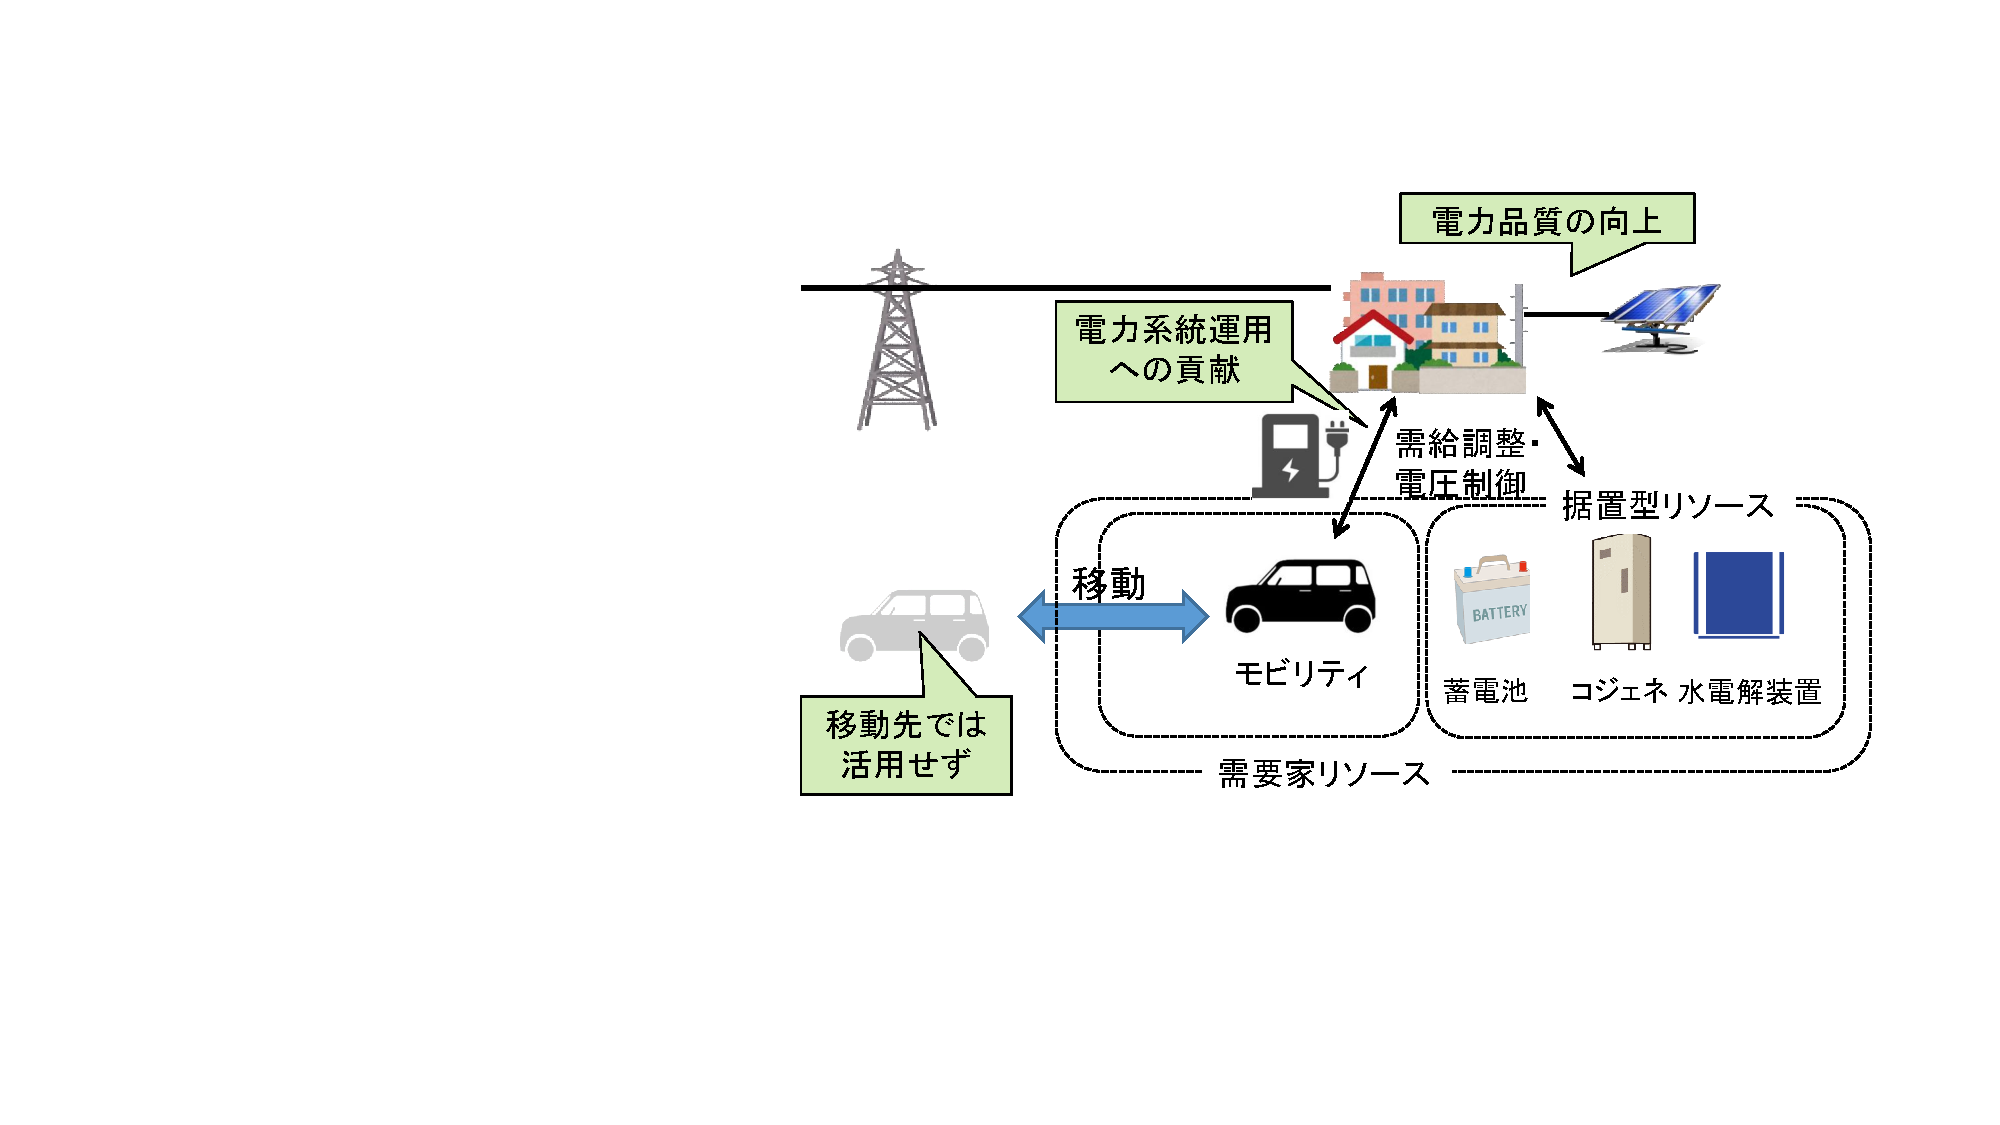
\includegraphics[width=9cm,height=5cm]{Summary_of_research_a.pdf}  
		  \caption{需要家リソースとの時間的な調整の活用イメージ}		  
		  \label{fig:Customer}
		\end{center}
		
%\end{wrapfigure}
%\begin{wrapfigure}{r}[0pt]{0.6\textwidth}
		\begin{center}
			\setlength{\abovecaptionskip}{0mm} % 図キャプション上空行幅調整
			  \setlength{\belowcaptionskip}{0mm} % 図キャプション下空行幅調整
			  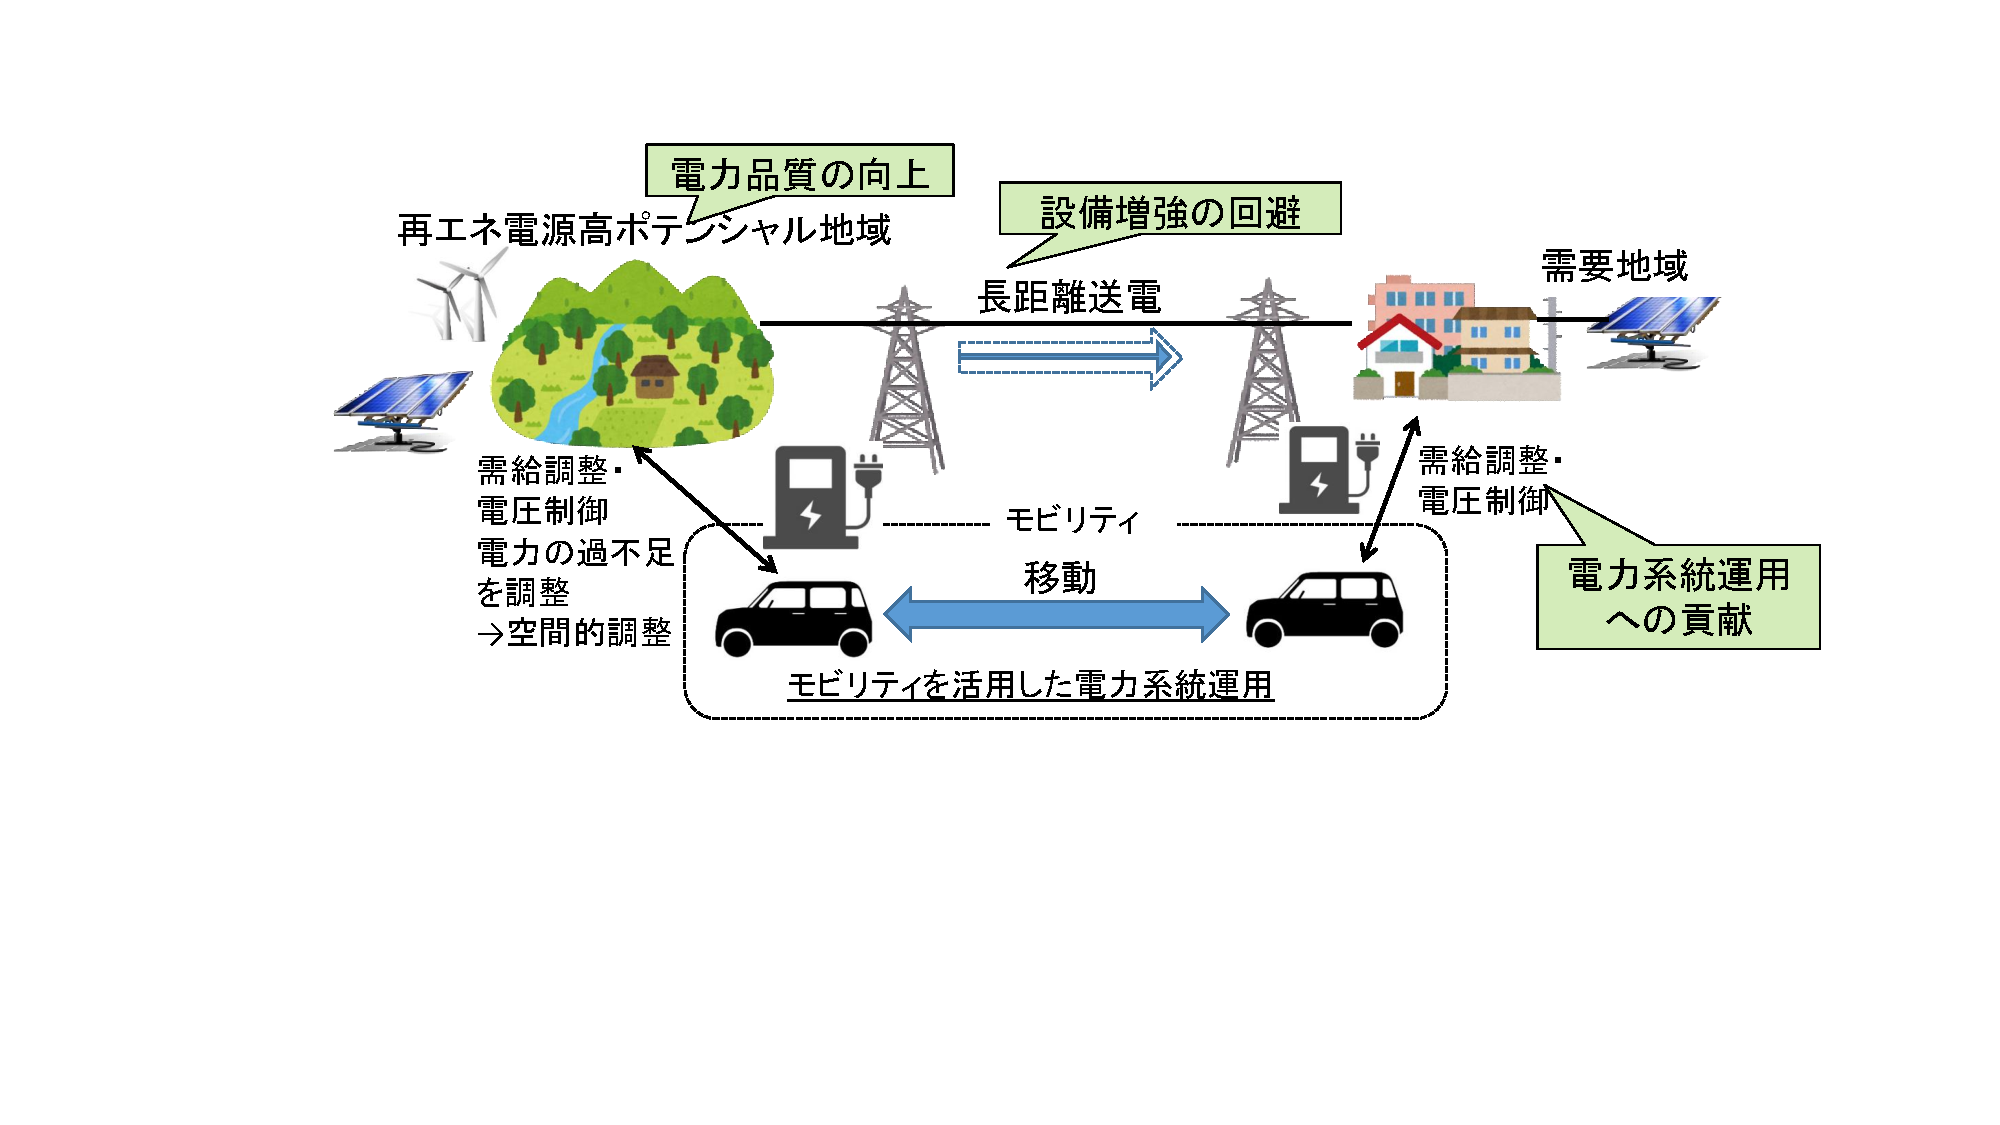
\includegraphics[width=11cm,height=5cm]{Summary_of_research_b.pdf}  
			  \caption{モビリティの空間的な調整の活用イメージ}
			  \label{fig:Mobility}
		\end{center}
\end{wrapfigure}
%\end{figure}


また,個々需要家リソースは,電力系統に対して容量が小さく,地理的に分散して電力システムに偏在している。
そのため,需要家リソースの活用に関しては,多数の需要家リソースを群として統括(アグリゲーション)する必要がある。
アグリゲーション技術としては,Virtual Power Plant (VPP) が注目を集めており,
申請者も据置型リソースでの時間的調整能力に準じたアグリゲーション技術について検討している。
しかしながら,モビリティの時空間的調整能力を電力系統運用に活かすための検討はなされていない。

\begin{enumerate}
	\setlength{\itemsep}{-5pt}
	\setcounter{enumi}{1}
	\paper{需給調整力提供を目的としたアグリゲータにより統括されるコージェネレーションシステムの最適運用}{\textbf{\ul{中村勇太}}, 他}{電気学会論文誌B}{139}{56-65}{2019}\label{pub:reg_by_CGS}
\end{enumerate}

また,我が国の電力システムにおいては,%前述した課題に加えて,%これと同時に,電力系統運用には新たな課題が浮上している。
(1)高度経済成長期に構築された設備の老朽化,
(2)田舎部をはじめとする人口減少地域における電力需要の減少,
(3)自然変動電源の大量導入された地域での電力余剰と電力消費が大きい都市部での電力不足といった
空間的な電力需要の不均衡の増大,等の要因から,
電力系統設備形成は大きな変革が求められている。
従来,電力設備形成は対象エリアの需要の大きさに対して,系統運用者側の設備が十分かといった観点で行われるが,
需要家リソースをはじめとする,需要家側の制御は想定されていない。

我が国の目標として,EVは2030年までに全自動車のうち30\%程度の販売数,
EV充電器は2030 年までに15万基(急速充電器3万基)の設置が見込まれており,
EVの電力需要量(kWh)およびEV用充電器(kVA)が電力系統全体に占める割合は,最大10\%程度とされている。
一方,一般的な電力系統の運用において,
需給調整に必要な能力量は総電力需要量の7\%程度,
電圧制御に用いられる静止型無効電力補償装置の容量は系統容量の10~20\%とされている。
モビリティの時空間調整により需要の不均衡を低減させることが可能であり,%自然変動電源の導入ポテンシャルが高い地域で発電した電力を電力消費地へエネルギー供給することが可能となり,
電力系統運用に必要な電力系統設備の容量削減といった,社会コストがより削減されるといった恩恵を得ることが期待できる(図\ref{fig:Mobility})。
そのため,\textbf{\ul{モビリティの電力系統運用貢献能力の大きさは電力系統の運用に必要な調整の大きさと同程度であり,
モビリティの活用により電力系統の最適な設備形成の在り方も変容する}}ことが予想される。

%この時間軸方向に関する制約を考慮し,需要家リソースを効果的に制御する方法が研究されている。
%申請者もこれまで,%電力系統運用に対する需要家リソースの貢献度を評価する手法を開発し,
%電力系統運用における需要家リソースの活用方法を検討してきた。
%最適化技術を用いて,
%需要家リソースの本来用途の利用や,
%貯蔵可能なエネルギー量に対する制約を考慮した,
%需要家リソースの貢献度を評価する手法を開発した。

%電動車の活用を最大限行うことで,電力系統運用に必要な設備の容量削減や設置回避が期待できる。

%申請者は,これまで
%そのため,%最適とされる運用を見つけ出すためには,
%モビリティを用いた検討は,時間的な調整あるいは空間的な調整のどちらか一方に着目した検討である。
%従来電源においては,発電出力の増減は出力可能範囲に限定されるものの,その増減状態を維持する継続時間は数秒~1時間以内の領域では制約にはならない。
%そのため,従来電源では調整するための幅($\Delta$kW) が重要であり,需給調整に関する学術的・実務的な検討の多くは,この$\Delta$kWに着目した議論である。
%一方,需要家リソースは瞬間的に調整する幅である$\Delta$kWに加えて,その幅を調整し続けることができる量$\Delta$ kW $\cdot$ h = $\Delta$ kWhに対する制約を考慮する必要がある。
%需要家リソースの設置・運用コストは未だ高いことから,
%需要家リソースからの調整力提供を自然変動電源による電力の需給バランス状況に合わせて調整する方法が研究されている。
%これに対しモビリティは,据置型リソースが提供可能な時間的な調整に加えて,
%自身の移動により,空間的な電力需給の調整も可能であるが,
%モビリティを用いた検討は,時間的な調整あるいは空間的な調整のどちらか一方に着目した検討である。
%この両者を同時に着目して需要家リソースを活用すると,

%モビリティを活用することで,




\vspace{-1\baselineskip}           %3. 上の余白
%\subsection*{(1)本研究の学術的背景、研究課題の核心をなす学術的「問い」}
\subsection*{(1-2)研究課題の核心をなす学術的「問い」}
\vspace{-0.5\baselineskip}           %3. 上の余白

%研究課題の核心をなす学術的「問い」は次の通りである。
\begin{itemize}
	\item \textbf{\ul{モビリティの時空間的調整能力の両者を電力系統運用の能力として評価するための,
	最適なアルゴリズムはどのようなものか?}}。

	\item \textbf{\ul{モビリティの時空間的調整能力の両者を効果的に電力系統運用に活用させるための
	最適な運用方法はどのようなものか?}}

	\item \textbf{\ul{需要家リソースの時空間的調整能力を効果的に活用した
	電力系統の最適な設備形成はどのようなものか?}}	
\end{itemize}


%\begin{figure}[h]
%    \begin{center}
    %\begin{minipage}%{8cm}
%      \begin{center}
%     \setlength{\abovecaptionskip}{0mm} % 図キャプション上空行幅調整
%      \setlength{\belowcaptionskip}{-5mm} % 図キャプション下空行幅調整
%      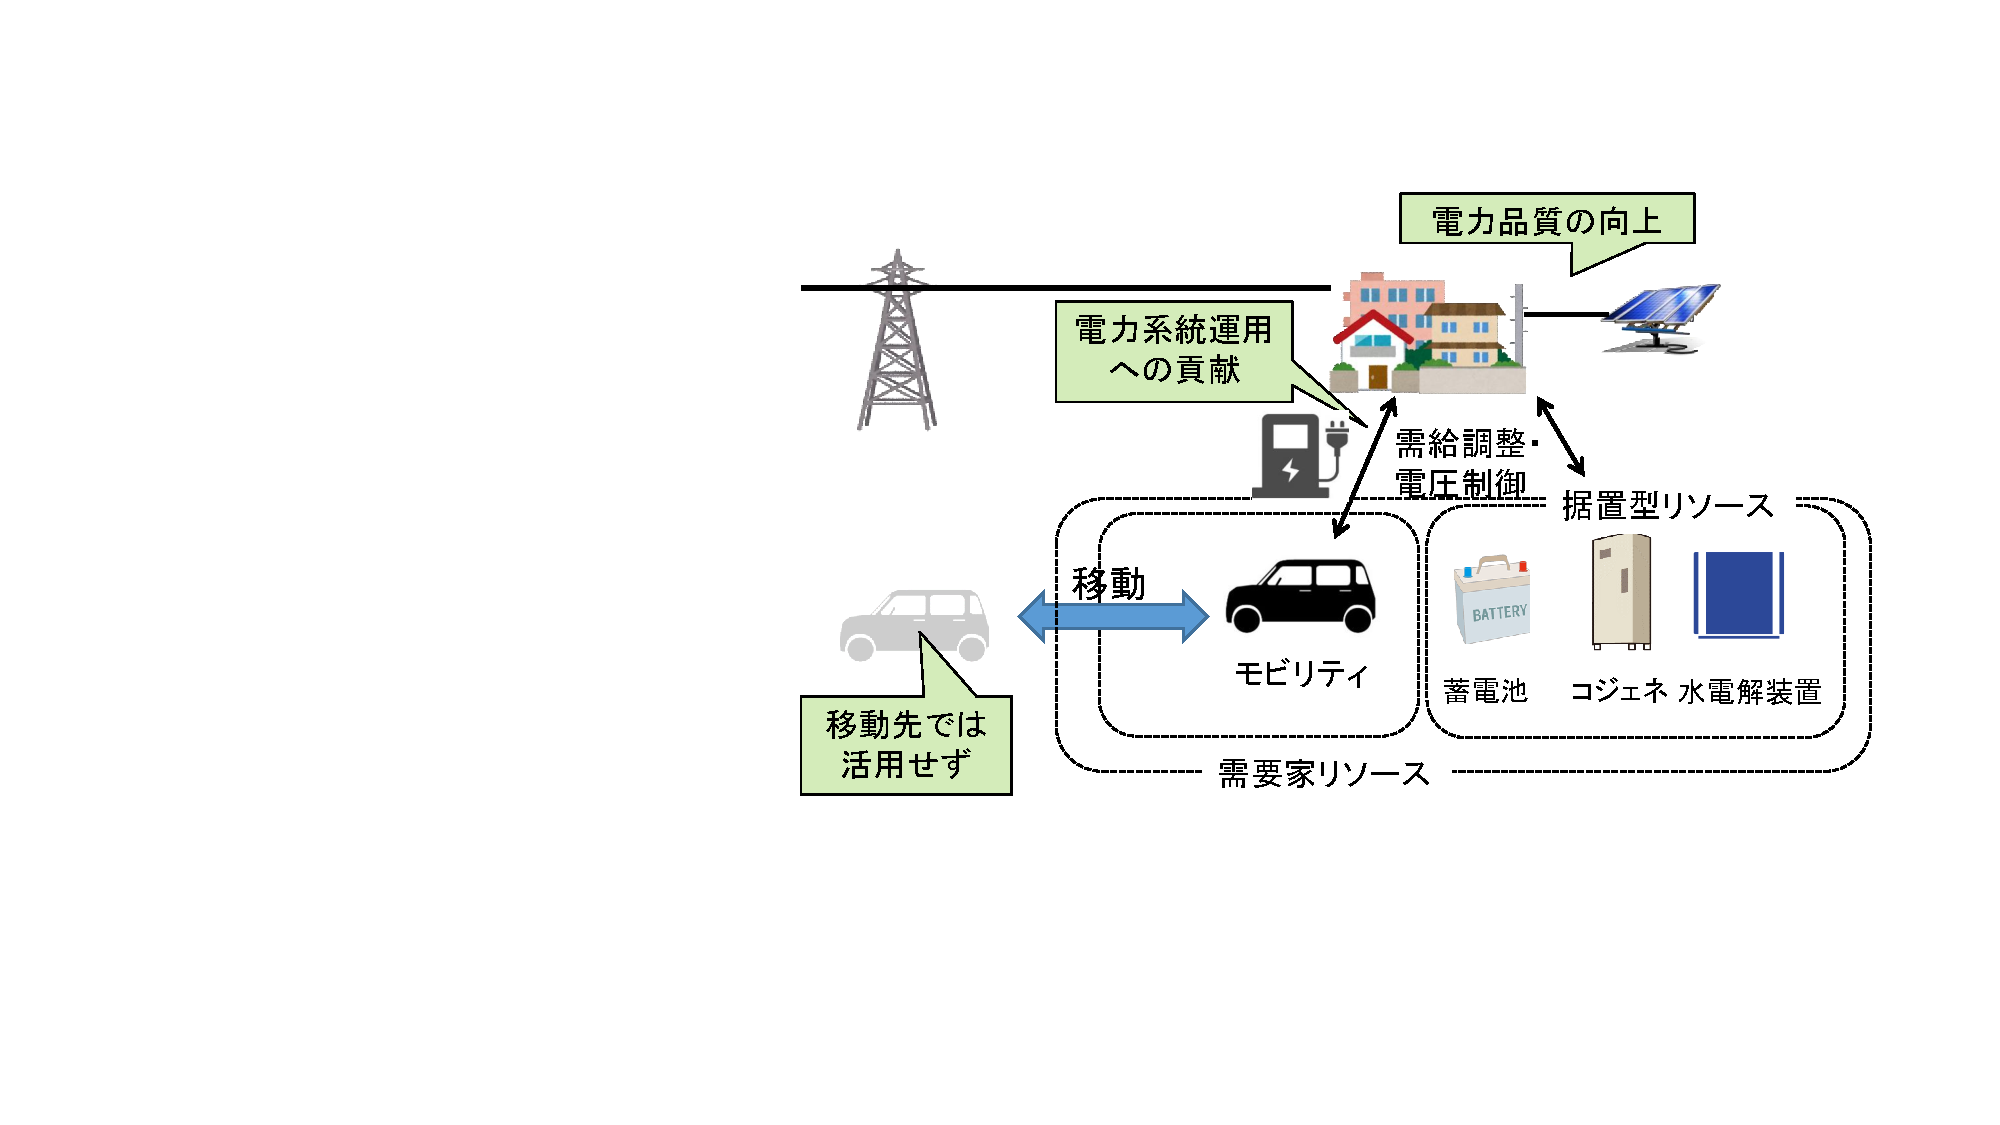
\includegraphics[width=14cm,height=4.5cm]{Summary_of_research_a.pdf}   
%      \subcaption{需要家リソースと従来の据置型リソースの活用イメージ}
%      \end{center}
    %\end{minipage}
  
    %\begin{minipage}%{8cm}
%      \begin{center}
%      \setlength{\abovecaptionskip}{-10mm} % 図キャプション上空行幅調整
%      \setlength{\belowcaptionskip}{-5mm} % 図キャプション下空行幅調整
%      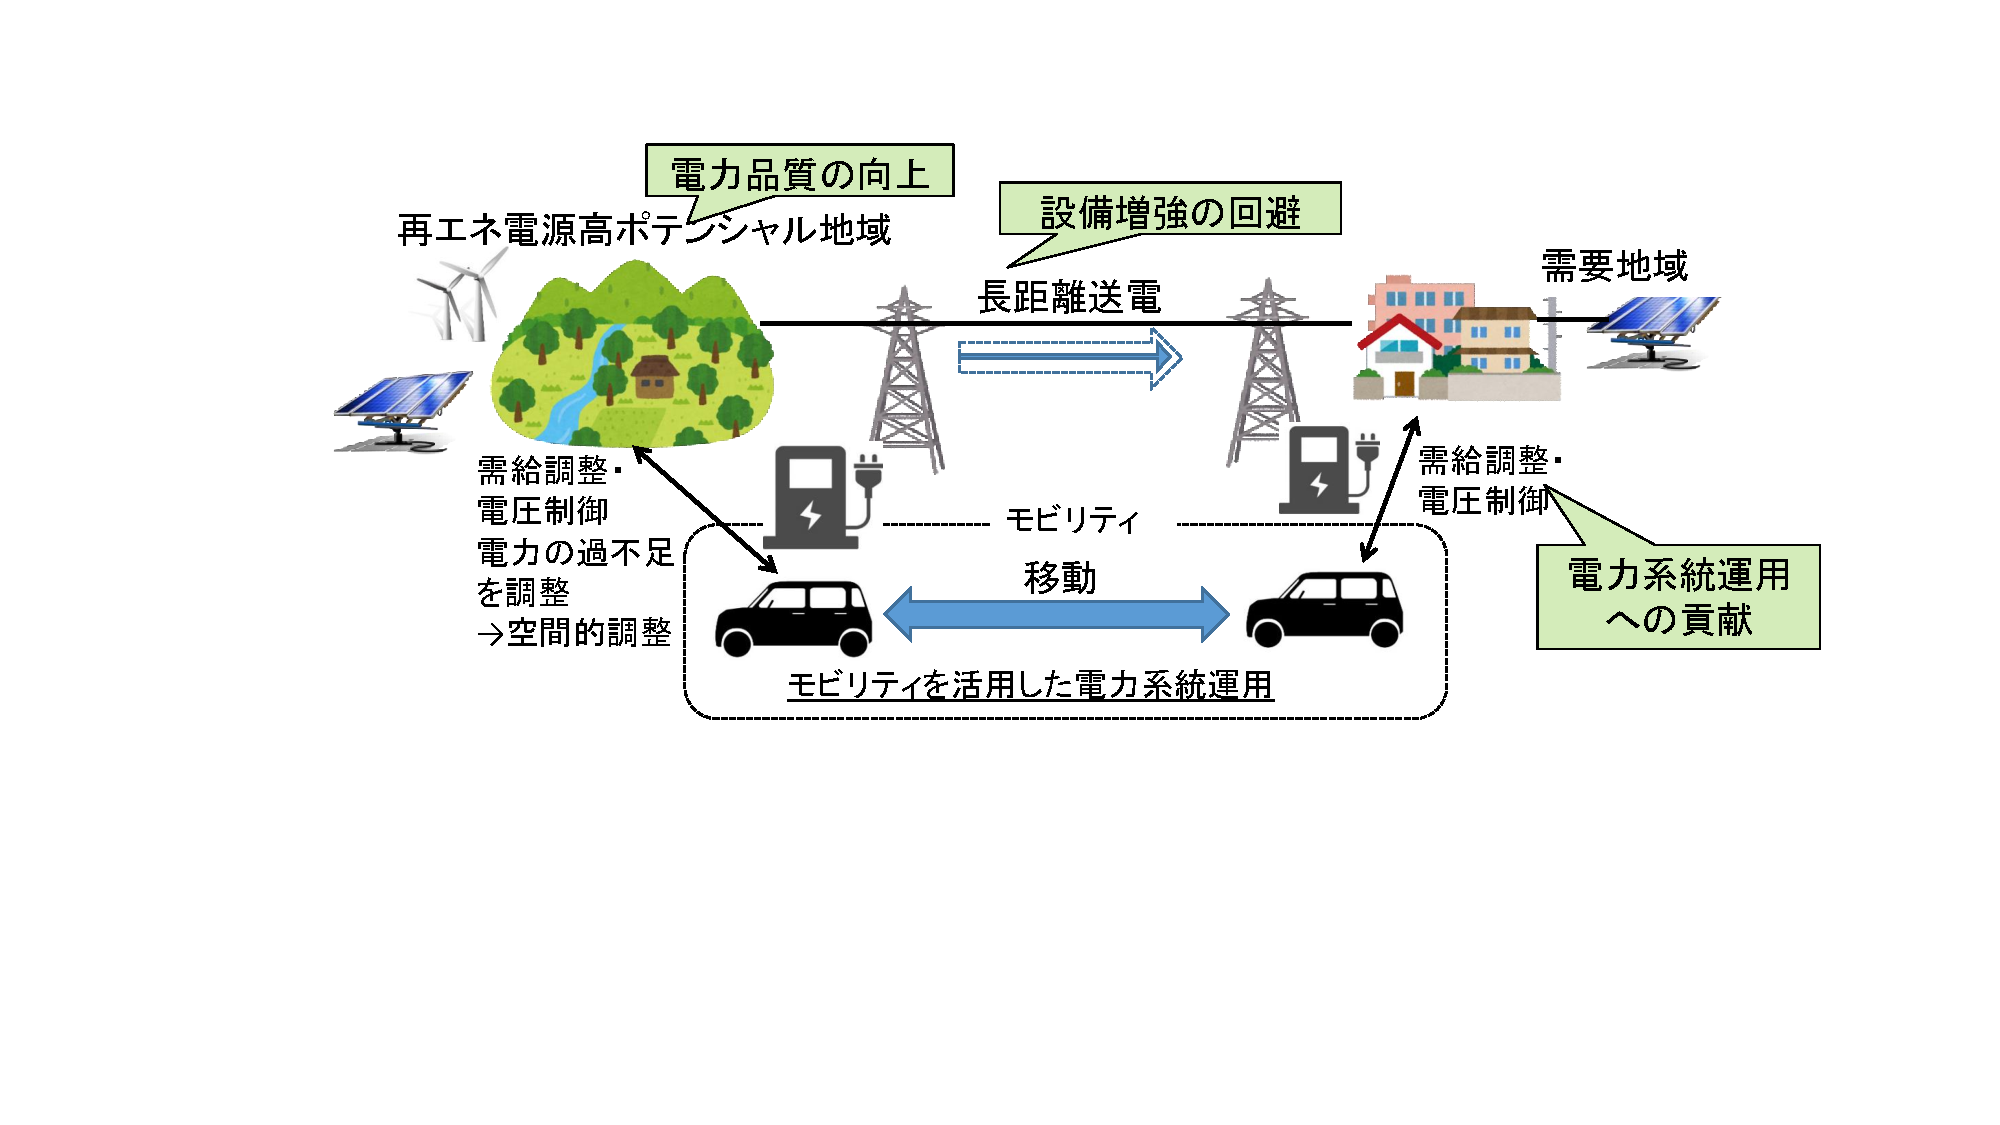
\includegraphics[width=14cm,height=4.5cm]{Summary_of_research_b.pdf}   
%      \subcaption{本研究で提唱するモビリティの活用イメージ}
%      \end{center}
    %\end{minipage}

%\begin{figure}[htbp]%{1.0\textwidth}
	%\centering
	  %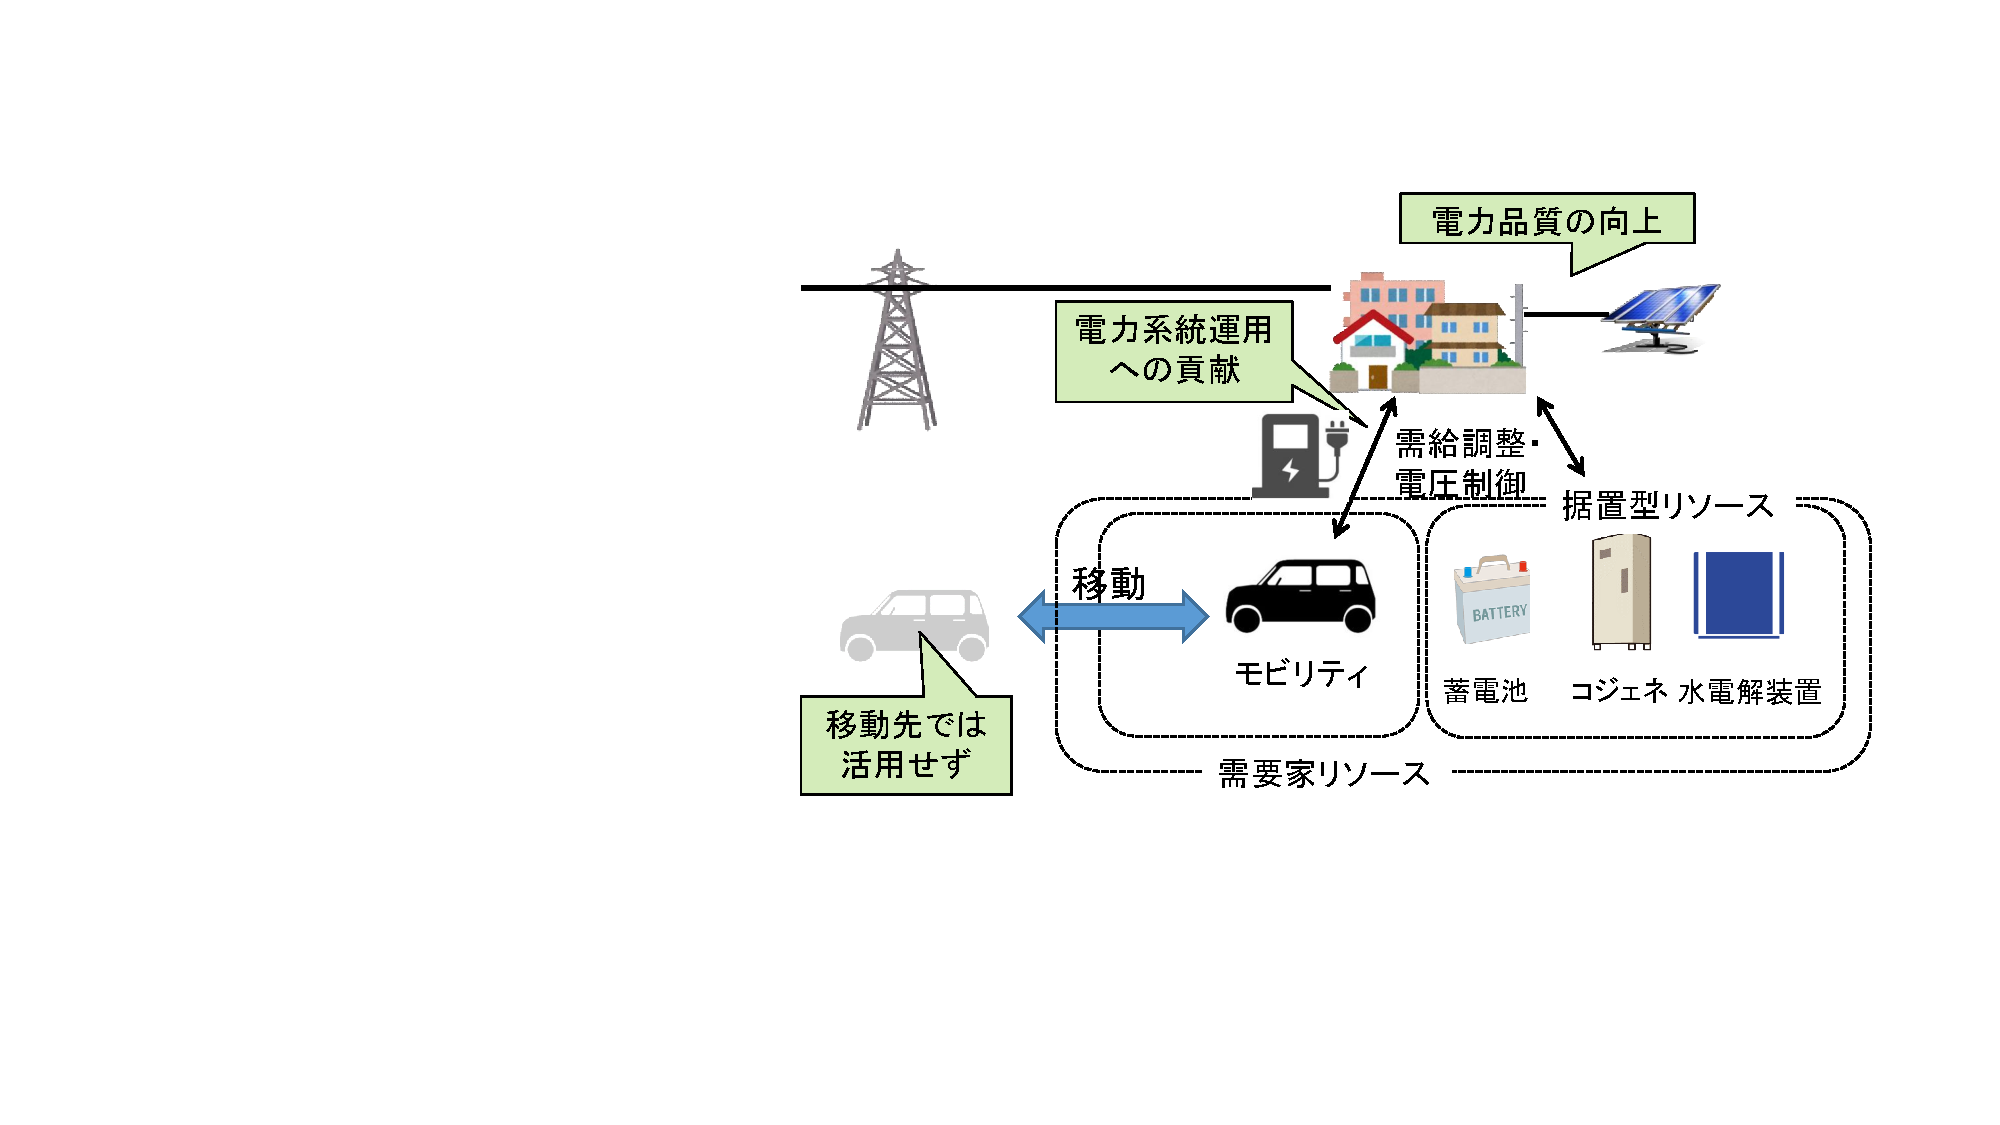
\includegraphics[width=16cm]{Summary_of_research_a.png}
%	\setlength{\abovecaptionskip}{0mm} % 図キャプション上空行幅調整
%    \setlength{\belowcaptionskip}{0mm} % 図キャプション下空行幅調整
%	\caption{需要家リソースを活用した電力系統運用のイメージ}
%	\label{fig:Summary}
%	\end{center}
%\end{figure}

%自然変動電源の導入による電力需要の減少や、高度経済成長期に構築された設備の老朽化が電力系統の運用に与える影響について、どのように対処すべきかが問われています。
%また、自然変動電源とモビリティの融合によって電力潮流が複雑化することで、電力品質の低下や設備容量の超過が懸念されています。

%本研究の核心的な学術的「問い」は、再生可能エネルギーを導入した電力系統の運用課題を解決し、
%持続可能なエネルギーシステムの構築に向けた手法を提案する。

%具体的には、自然変動電源とモビリティを融合した電力系統設備形成の新たなアプローチによって、
%電力供給の安定性と経済性を両立させることが、私たちの研究の根本的な問いとなります。

\vspace{-1.5\baselineskip}           %3. 上の余白
\subsection*{(2-1)本研究の目的}
%\subsection*{(2)本研究の目的及び学術的独自性と創造性}
\vspace{-0.5\baselineskip}           %3. 上の余白

本研究では,(1)で述べた事項を踏まえ,下記を確立することを目的とする。
\begin{itemize}
	\item \textbf{[項目1]}モビリティが有する空間的な調整を正確に評価する方法
	\item \textbf{[項目2]}モビリティを最大限活用するためのアグリゲート手法
	\item \textbf{[項目3]}需要家リソースの時空間的な調整を活用した電力系統の設備形成の在り方
\end{itemize}


%\subsubsection*{時空間的な需給調整能力を定量的に評価する手法の確立}
\vspace{-1.5\baselineskip}           %3. 上の余白
\subsection*{(2-2)学術的独自性と創造性}
%\subsection*{(2)本研究の目的及び}
\vspace{-0.5\baselineskip}           %3. 上の余白

据置型リソースは,時間的な需給調整能力をその機器容量や電力の調整幅として評価することができるが,
モビリティによる空間的な調整は,据置型リソースと同様の時間軸方向の制約に加えて,
電気的・地理的位置および各地点の再エネ電源や負荷需要といった系統状況により変化するため,
単純に評価することはできない。
また,関連する検討では,系統全体として電力系統運用に必要な調整に対して,
需要家リソースが提供する調整が十分かといった観点で取り扱われてきた。
しかしながら,\textbf{\ul{モビリティは,系統の地点で異なる電力系統運用に必要な調整能力に対して,
調整能力を柔軟にマッチング}}させることが可能である。

このように,\textbf{\ul{電力系統および需要家リソースの間で調整能力のマッチングを積極的に行う事例はなく,
これ自身が独自性・創造性の高い内容}}であるといえる。
%電力系統をより柔軟かつ効果的に運用することが可能となることが期待される。
%\textbf{\ul{時空間的な調整能力を定量的に評価する手法を確立することは,それ自身が独自性の高い内容であるとともに,
%電力系統の運用・設備形成に関する適用範囲が広く,有用性も高い}}ものとなるといえる。
%電力系統に連系される自然変動電源およびモビリティが増加していく中で,
%モビリティは,%これに加えて,リソース自身の移動による空間的な調整能力を考慮する必要があり,



%その評価に基づき,モビリティを効果的な電力系統運用手法の確立(\textbf{[項目2]})も本研究の目的である。

%\textbf{\ul{モビリティの空間的な調整能力も考慮したアグリゲーションに関する検討例はなく,
%本研究の成果をもって,実系統における需要家リソースの活用能力をより正確に評価し,
%需要家リソースの付加価値向上に寄与}}することが期待される。

%また,モビリティを効果的に活用した電力設備形成の検討(\textbf{[項目3]})も本研究の目的である。
%さらに需要家リソースを活用することで,需要家リソース自身が連系されている電力系統の設備形成にも貢献することが期待される。
%据置型およびモビリティの両者の特性を活かし統合的に活用することで,
%自然変動電源の導入ポテンシャルが高い地域で発電した電力を電力消費地へエネルギー供給することが可能となり,
%本来必要な長距離送電容量や据置型リソース容量の削減効果が期待できる。
%しかしながら,現状では電力系統の設備形成への貢献を前提とした需要家リソースの活用は,
%前述した据置型リソースが有する時間的な調整に基づくものであり,
%モビリティの空間的な調整も考慮した検討はなされていない。
%自然変動電源の導入と共に人口減少や過疎化が進む我が国において,
%\textbf{\ul{自然変動電源に加えて需要家リソースを最大限活用した電力系統の設備形成の在り方を検討することは,
%世界の電力システムにおける将来の電力系統設備形成において極めて重要}}となり得る。

%\subsubsection*{(3)本研究の着想に至った経緯と}
\vspace{-1\baselineskip}           %3. 上の余白
\subsubsection*{(3-1)本研究の着想に至った経緯}
\vspace{-0.5\baselineskip}           %3. 上の余白

申請者はこれまで,%蓄電池やコージェネレーションシステム(コジェネ),水電解装置といった
据置型リソースを対象に,電力系統運用に貢献する手法について検討してきた。
据置型リソースの多くは制御性に優れており,電力系統の運用において一定の貢献が期待できるものの,
据置型リソースの多くが設備容量が小さく,導入量はまだ限定的であることから,
電力系統運用に与えるインパクトは依然として小さい。
その中で,近年ではモビリティである電気自動車をはじめとするモビリティが飛躍的に普及している。
モビリティは据置型リソースよりも大容量のものが多く,据置型リソースと同様の活用に加え,
移動により電力需要バランスおよび各地点における電力系統運用への調整能力を空間的に調整できるなど,
電力系統運用に対してより柔軟かつ効果的に貢献できることが期待される。
\textbf{\ul{しかしながら,モビリティを電力系統運用として検討されているほとんどが据置型リソースと同様の活用であり,
モビリティが特定の系統に連系されたときにしか活用されていない}}。

また,モビリティに関しては自動運転技術が飛躍的に進んでおり,
将来的に無人で荷物を運搬することが当たり前となってくることが予想される。
その自動運転時に,人や荷物の運搬といった本来用途に加えて,
電力系統に貢献するリソース活用を融通することで,
系統全体の運用や系統設備形成が最適化されるのではないかと着想した。

%モビリティは,移動することが本来の目的であるため,
%移動中は電力系統運用に貢献できないなど,
%より適切に運用しなければ調整能力が大きく制限されてしまう。
%同規模の据置型リソースに比べて時間的な制約により活用能力は制限される。
%そのため,その特徴を反映した定量的な能力評価手法を確立するとともに,
%据置型リソースとの能力との棲み分け方を明確にすることが重要であると考え,本研究を着想した。
%さらにモビリティは,電力系統間の電力・調整能力偏りを解消する空間的な調整ポテンシャルを有していると想定されるため,
%電力系統設備形成の在り方も大きく変えることができると考え,本研究を着想した。

\vspace{-1\baselineskip}           %3. 上の余白
\subsubsection*{(3-2)関連する国内外の研究動向と本研究の位置づけ}
\vspace{-0.5\baselineskip}           %3. 上の余白

電力系統運用に対する需要家リソースの活用は欧米を中心に検討・導入され,
近年は,再生可能エネルギーの大量導入による余剰電力対策としても注目されている。
最近は,ITとの融合を目指したスマートグリッド技術の一要素として,
系統側の状況に合わせて需要を能動的に制御する考え方は浸透しつつある。
我が国においても,%再生可能エネルギーの導入増加を背景に,
需要抑制量を発電機の発電量に見立てて取引するネガワット取引や,
電力需給調整市場取引などが注目を集めており,
\textbf{需要家リソースは従来電源とともに,
これらの取引の中心的な役割}を担うことが期待されている。
%また,モビリティの代表例である電気自動車も
%電力系統運用に貢献することが期待されている。

%その中でも,据置型およびモビリティの両者が対象とされているが,
その一方で,検討されている需要家リソース活用は,%需要家リソースの物理的な位置および連系されている系統の状況については考慮されておらず,
電力需給といった系統全体としては最適な運用や制御がなされるものの,
系統単位といった観点では,空間的調整が十分活用されていないため,
モビリティの活用能力を最大限に引き出せていない。
%需要家リソースが連系されている系統内の状態といったローカルな観点では最適制御がされていない(図\ref{fig:Summary}(a))。
\textbf{\ul{モビリティが接続されている系統を逐次把握し,全体として最適な運用や制御を行うといった,
需要家リソースの活用能力評価や運用・アグリゲーションに関する研究事例}}(図\ref{fig:Mobility})
\textbf{\ul{はなく,本研究で先駆けて提唱する}}ものである。


\vspace{-1\baselineskip}           %3. 上の余白
\subsection*{(4)本研究で何をどのように、どこまで明らかにしようとするのか}
\vspace{-0.5\baselineskip}           %3. 上の余白

\vspace{0.5\baselineskip}           %3. 上の余白
\textbf{[項目1]モビリティの時空間的な調整能力評価(2024年度):}
%EVを対象に,モビリティの時空間的な調整能力を評価する手法を開発する。
各種リソースを有する需要家の%電気や熱といった
エネルギーフローおよびモビリティの移動の起点・終点の位置や移動時間を考慮した上で,
出力調整の大きさと調整時間から需給調整能力を評価する。%($\Delta$kW)
この評価のため,電力系統における電圧や電力潮流量に関する制約を主問題,
各需要家・各需要家リソースにおけるエネルギーフローや調整幅に関する制約を副問題とする多レベル最適化問題として定式化・求解する。
%この評価は,特に電力系統内の状況やモビリティの移動トリップの状況に応じて変化するため,
%これらを統計値として確率論的アプローチを用いて行う。
%自然変動電源の発電状況や移動トリップを確率論的アプローチによって取り扱う。

% 削除候補段落
%また,需要家リソース自身とその他の設備容量,モビリティの移動タイミングをパラメータとして感度分析を実施することで,
%これらの要因が調整能力に与える支配的な要因を明らかにする。
%この結果は,項目2,項目3の実施内容で想定する各需要家リソースの活用手法の基盤となる。

\vspace{0.5\baselineskip}           %3. 上の余白

\textbf{[項目2]モビリティを効果的に活用した電力系統運用(2025年度~2026年度前半):} 
\textbf{[項目1]}の活用能力評価を元に,モビリティを効果的に活用した電力系統運用を開発する。
%具体的には,
%アグリゲーション対象の%手法は,需要家リソースを有する需要家のエネルギーモデルを統合的に束ねて制御することであるが,
%需要家リソースは系統に多数,偏在的に存在しているため,
実際の電力系統運用を想定した場合,
電力系統運用者が,需要家の需要に関する情報を全て把握し,
電力系統設備や需要家リソースの運用を決定することは現実的ではない。
%さらに,そのため,\textbf{[項目1]}で
%\textbf{[項目1]}で述べた最適化問題を定式化し,
%工学的に実用的な時間で適切な解を求めることは,現実的ではない。
そこで,\textbf{[項目1]}の最適化問題を緩和し,
電力系統運用者と需要家の間で時空間的調整能力をマッチングさせ,
実用的な計算量で可搬型および据置型リソース群をアグリゲートする,
電力系統運用手法を開発する。

\vspace{0.5\baselineskip}           %3. 上の余白

\textbf{[項目3]モビリティを効果的に活用した電力設備形成の在り方(2026年度~2027年度):} 
%\textbf{[項目2]}の電力系統運用手法に従う電力設備形成について検討する。
%実際の電力設備形成は,様々な事情や要因によって異なるため一般性を持たないことが多いが,
%\textbf{[項目1]}により得られた知見を元に,
%電力系統に導入されている自然変動電源の容量や割合や,需要家リソースの種類や個数,
%モビリティの場合は移動トリップ状況などの要素が,
%最適な電力設備形成にどう影響を与えるか,といった設備形成を検討するための方針・モデルを確立する。
\textbf{[項目2]}で確立した電力系統運用手法において,
自然変動電源・需要家リソースの個数・容量や,
電力系統運用に関する制約(電圧制御や潮流量制約)の上下限値をパラメータとして変化させ,
需要家リソースの活用および電力系統内の電圧機器や調相の制御に関する感度解析を行う。
この感度解析結果から得られる需要家リソース活用による経済的恩恵,
および電力系統の設備構成の設置や維持に関する費用から,
据置型および可搬型リソースを効果的に活用した電力設備形成の在り方について明確化する。


%\begin{table}[htbp]%{1.0\textwidth}
%	\setlength{\abovecaptionskip}{0mm} % 図キャプション上空行幅調整
%   \setlength{\belowcaptionskip}{0mm} % 図キャプション下空行幅調整
%	\caption{研究項目と研究計画}
%	\label{fig:test}
%	\centering
%	  \includegraphics[width=16cm]{Roadmap_of_research.png}	
%\end{table}


\vspace{-1\baselineskip}           %3. 上の余白
\subsection*{(5)本研究の目的を達成するための準備状況}
\vspace{-0.5\baselineskip}           %3. 上の余白

%蓄電池やコジェネ,水電解装置を対象とした,
%2-(1)で示すように,
\textbf{[項目1]}および\textbf{[項目2]}について,
据置型リソースに関する調整能力評価および活用手法に関する研究は,
これまでの検討により一定の成果が得られている。%,また,耐災害性に対する活用なども検討しており,
%これまでの検討で定式化した最適化問題に,
%モビリティ特有の移動に関する制約を新たに考慮することで,
%空間的な調整能力の評価や効果的な活用が可能になることが見込まれる。
%また,%据置型リソースの調整能力を
%電圧制御や災害時の電力供給や%に活用するための需要家側の運用,
%配電線のスリム化といった電力設備形成に関する研究など,
%様々な目的に対する需要家リソースの運用手法に関する検討を行っている。
また申請者は本学の学内研究推進経費(2023年度)に採択され,モビリティであるEVに着目し,
単独の系統において,
系統運用の必要な調整能力とモビリティの調整能力をマッチングさせるための概念に関する検討を行っている。
配電系統における配電線をなくし,エネルギーの自給自足を行う
「電力系統のオフグリッド化」を実現するための各種設計といった,
電力設備形成に関する検討も行っている。
ぞのため,\textbf{[項目3]}についても,%据置型リソースを活用した配電線のスリム化や,
電力系統のオフグリッド化にあたり得られた知見を本研究に活かすことで,
可搬型および据置型の両者の需要家リソースを対象とした電力設備形成の在り方も確立できると考えている。



	%\vspace{1cm}
	%\begin{thebibliography}{99}
		%\bibitem{teramura} 寺村輝夫、「ぼくは王様 - ぞうのたまごのたまごやき」.
	%\end{thebibliography}
%end 研究目的と研究計画 ====================

% p01_purpose_plan_01.tex
\KLEndSubject{F}


%#Split: 03_abilities  
%#PieceName: p03_abilities
% p03_abilities_00.tex
\KLBeginSubject{02}{2}{2 応募者の研究遂行能力及び研究環境}{2}{F}{}{jsps-subject-header}{jsps-default-header}

\section{2 応募者の研究遂行能力及び研究環境}
%    <<最大 2ページ>>

% s14_abilities
%\PapersInstructions		% <-- 留意事項。これは消すか、コメントアウトしてください。
%begin 応募者の研究遂行能力及び研究環境 ====================

\vspace{-2\baselineskip}           %3. 上の余白
\subsection*{(1) これまでの研究活動}
\vspace{-0.5\baselineskip}           %3. 上の余白

	申請者はこれまで,電力系統運用に貢献する需要家リソースの活用に関する検討を行ってきた。
	以下に,本研究の各項目に対応させて示す。

	\vspace{-1.5\baselineskip}           %3. 上の余白
	\subsubsection*{\textbf{[項目1]} モビリティの時空間的な調整能力評価}
	\vspace{-0.5\baselineskip}           %3. 上の余白

	%中部電力(株),中部電力パワーグリッド(株)との共同研究を通じて,
	据置型リソースである蓄電池を用いた需給調整提供に関する検討[\ref{pub:voltage_reg_by_bat}]では,
	蓄電池の時間的な制約を考慮した,需要家リソースを有する需要家単位で最適化問題を解くことで,
	時間的な調整能力を評価する手法を開発した。
	この手法は,事前に調整の継続時間を決め,その時間にしたがって調整した際のエネルギー量の制約を考慮しつつ,
	調整の大きさを最大化する手法である。	

	水電解装置を用いた需給調整提供,電圧制御を考慮した運用手法[\ref{pub:reg_vol_by_MG}]について検討した。
	検討した手法は,単独の系統において,需要家のエネルギー需要や本来の用途(水素生成)を考慮し,
	需給調整力提供および電圧制御のための無効電力供給による報奨金(対価)を含めた,
	運用コスト(費用)が最小となるような運用を最適化計算によって決定する手法である。
	この手法により,複数の電力系統運用への貢献能力を評価でき,
	据置型リソースを最適に運用することが可能となる。	

	また,電圧制御に貢献する運用手法に関する検討[\ref{pub:RA_by_bat}]では,
	単独の電力系統における単独の蓄電池・充電器を対象に,
	時間的な調整を電力系統電圧制御に最大に活用するための運用手法を開発した。
	この手法は,電力系統に関する制約として,電力系統内の潮流量制約や潮流方程式を考慮し,
	電圧変動を最小化するように蓄電池の出力を決定する手法である。
	EV用急速充電器による配電系統の電圧制御手法[\ref{pub:voltage_by_EV}]を開発した。
	この手法は,充電器の空き容量を電力系統の電圧制御に活用するための運用手法であり,
	本研究では,電力系統に接続されている充電器はこの手法を前提として運用されることで,電力系統運用に貢献する。

	さらに,蓄電池やコジェネ,水電解装置,燃料電池といった複数の需要家リソースを有するマイクログリッドを想定し,
	マイクログリッドの運用手法[\ref{pub:hybrid}]について検討した。
	この検討では,マイクログリッドの運用を策定するにあたり最適化問題を解いているが,
	その最適化解法のアプローチは,
	厳密解ではないが,効果的に解を近似的に探索するMILP(Mixed Integer Linear Programming)の最適化と,
	時間がかかるが厳密解を求めることができる粒子群最適化(PSO: Particle Swarm Optimization)を組み合わせたハイブリッド手法であり,
	\textbf{[項目1]}や\textbf{[項目2]}での最適化問題を効果的に解く,計算技術の基盤となる。


	\vspace{-0.5\baselineskip}           %3. 上の余白
	\begin{enumerate}
		\setlength{\itemsep}{-5pt}
		\paper{Study on Operation in Power System Utilizing Customer's Resource for Providing Demand and Supply Regulation}{\textbf{\ul{Y.Nakamura}}, et al.}{2020 International Conference on Smart Grids and Energy Systems}{(SGES)}{66-70}{2020}\label{pub:voltage_reg_by_bat}
		
		\paper{電力系統運用に貢献する水素供給設備を含むマイクログリッドの運用に関する検討}{\textbf{\ul{中村勇太}},青木睦,加戸良英,壹岐浩幸}{電気学会論文誌B}{141}{56-66}{2021}\label{pub:reg_vol_by_MG}

		%M.Aoki and S.C.Verma
		\paper{Optimal Charging Method for Batteries in Distribution System to Supply Demand in Remote Area}{\textbf{\ul{Y.Nakamura}}, et al.}{CIGRE 2022 Kyoto Symposium}{19-4}{111}{2022}\label{pub:RA_by_bat}
		%M.Aoki, K.Hikoyama and T.Nonoyama

		%\paper{電圧制御機器のタップ切替動作削減に貢献する蓄電池群の運用および必要容量評価に関する検討}{\textbf{\ul{中村勇太}},青木睦,金沢由樹,上西宏和}{電気学会論文誌B}{140}{474-483}{2020}\label{pub:voltage_by_bat}

		%\paper{遠隔地のオフグリッド化に貢献する蓄電池充電に関する検討-充電設備の位置および利用状況が充電特性に与える影響-}{\textbf{\ul{中村勇太}},青木睦, 彦山和久, 野々山公亮}{電気学会電力技術/電力系統技術合同研究会}{PE-21-085}{PSE-21-098}{2021}\label{pub:cha_by_bat}
	
		\paper{配電系統における電気自動車用急速充電器を用いた電圧制御}{\textbf{\ul{中村勇太}}, 原亮一, 北裕幸, 田中英一}{電気学会論文誌B}{138}{107-115}{2018}\label{pub:voltage_by_EV}

		%\paper{Novel Optimization Method Hybridized by MILP and PSO for Operation Planning in Microgrid System}{Y.Tanahashi, H.Kobayashi, \textbf{\ul{Y.Nakamura}},M.Aoki}{International Power Electronics Conference 2022}{(IPEC-2022)}{1359-1364}{2022}\label{pub:MILP_PSO}

		\paper{マイクログリッドシステムの運転におけるMILPとPSOを用いたハイブリッド手法の実用性評価}{棚橋優, 小林浩,\textbf{\ul{中村勇太}},青木睦}{電気学会論文誌D}{142}{897-906}{2022}\label{pub:hybrid}
	\end{enumerate}

	\vspace{-1.5\baselineskip}           %3. 上の余白
	\subsubsection*{\textbf{[項目2]} モビリティを効果的に活用した電力系統運用}
	\vspace{-0.5\baselineskip}           %3. 上の余白

	%コジェネを用いた需給調整提供および設備容量設計[\ref{pub:design_by_CGS}],
    文献[\ref{pub:reg_by_CGS}]ではコジェネ群をVPPとみなし,
	全体としてどのようにアグリゲートするかといった運用手法について検討した。
	検討した手法は,コジェネを統括するアグリゲータ(系統側)が各コジェネ(需要家側)に対して,
	必要な調整能力(上限)を提示し,各コジェネからその能力を受け取ることで,
	全体として必要な能力を確保する手法である。
	\textbf{[項目1]} に関する手法[\ref{pub:reg_vol_by_MG}]
	において,対象となる系統が複数になる点が,本研究の\textbf{[項目2]}における系統運用手法に相違点となる。%が,
	%この研究で得られた知見が生かせると期待される。

	パワーアカデミー研究助成[\ref{pub:PA_2017}]において,
	需給調整を目的としたリソース活用時に需要家の本来用途の変化(不確実性)
	が与える影響を考慮した系統運用手法について検討した。
	この不確実性の考慮は,本研究の\textbf{[項目2]}における系統運用手法においても必要となる。

	\vspace{-0.5\baselineskip}           %3. 上の余白
	\begin{enumerate}
		\setlength{\itemsep}{-5pt}

		\setcounter{enumi}{5}
		%\paper{Study on Operation in Power System Utilizing Customer's Resource for Providing Demand and Supply Regulation}{\textbf{\ul{Y.Nakamura}},M.Aoki and S.C.Verma}{2020 International Conference on Smart Grids and Energy Systems}{(SGES)}{66-70}{2020}\label{pub:voltage_reg_by_bat}

		%\paper{Optimal Charging Method for Batteries in Distribution System to Supply Demand in Remote Area}{\textbf{\ul{Y.Nakamura}}, M.Aoki, K.Hikoyama and T.Nonoyama}{CIGRE 2022 Kyoto Symposium}{19-4}{111}{2022}\label{pub:RA_by_bat}
		\paper{需給調整力提供を目的としたアグリゲータにより統括されるコージェネレーションシステムの最適運用}{\textbf{\ul{中村勇太}}, 原亮一, 北裕幸, 武田清賢}{電気学会論文誌B}{139}{56-65}{2019}\label{pub:reg_by_CGS}

		
		\paper{需要家リソースを活用したスマート型電力システムの確率的系統運用手法}{\textbf{\ul{中村勇太}}}{パワーアカデミー研究助成萌芽研究博士課程枠}{}{}{2017}\label{pub:PA_2017}
		

	\end{enumerate}


	\vspace{-1.5\baselineskip}           %3. 上の余白
	\subsubsection*{\textbf{[項目3]} モビリティを効果的に活用した電力設備形成の在り方}
	\vspace{-0.5\baselineskip}           %3. 上の余白

	電力設備形成に関連して,
	%蓄電池の時間的な調整による活用を前提とした電力設備形成の在り方として,
	文献[\ref{pub:voltage_by_bat}]では無効電力補償装置,
	文献[\ref{pub:slim_by_bat}]では配電線
	の容量削減や増設回避に関する検討を行っている。%,配電線撤去の実現可能性)
	これらの検討では,需要家リソースの活用能力を%設備形成を検討するにあたり,
	特有の時間的な制約を考慮した無効電力補償装置や配電線の等価的な容量として評価している。
	また,文献[\ref{pub:design_by_CGS}]では,需要家リソースの容量を変化させた際の活用能力評価・容量設計を行っている。
	%\ref{pub:cha_by_bat}]について検討しており,
	配電系統を対象に,EVによる空間的な調整を活用した電力設備形成に関する検討[\ref{pub:OG_by_EV}]を行っており,
	電力系統の配電線撤去に必要なEVの台数や,その経済的効果について試算を行った。	

	\textbf{[項目3]}モビリティによる時空間的調整を考慮した電力系統設備および需要家リソースの容量設計といった電力系統設備形成を検討するにあたり,
	これらの検討で得られた知見が欠かせない。
	
	%また,水電解装置を電力需給調整市場に参加させることで得られる経済的恩恵についても定量的に示しており[\ref{pub:cost_by_MG}],
	%需要家リソースを電力系統運用に活用することの有効性を示している。

	\vspace{-0.5\baselineskip}           %3. 上の余白
	
	\begin{enumerate}
		\setlength{\itemsep}{-5pt}
		\setcounter{enumi}{7}

		\paper{電圧制御機器のタップ切替動作削減に貢献する蓄電池群の運用および必要容量評価に関する検討}{\textbf{\ul{中村勇太}},青木睦,金沢由樹,上西宏和}{電気学会論文誌B}{140}{474-483}{2020}\label{pub:voltage_by_bat}
		
		\paper{配電線スリム化を目的としたダイナミックレーティング適用時の蓄電池設備容量評価}{石田匠輝,\textbf{\ul{中村勇太}},青木睦, 彦山和久, 野々山公亮}{電気学会論文誌B}{143}{379-388}{2023}\label{pub:slim_by_bat}

		\paper{需給調整に貢献するコージェネレーションシステムの設備設計に関する検討}{\textbf{\ul{中村勇太}}, 原亮一, 北裕幸, 武田清賢}{電気学会論文誌B}{140}{219-228}{2020}\label{pub:design_by_CGS}
		
		%\paper{遠隔地のオフグリッド化に貢献する蓄電池充電に関する検討-充電設備の位置および利用状況が充電特性に与える影響-}{\textbf{\ul{中村勇太}},青木睦, 彦山和久, 野々山公亮}{電気学会電力技術/電力系統技術合同研究会}{PE-21-085}{PSE-21-098}{2021}\label{pub:cha_by_bat}

		\paper{配電系統における最適充電制御される電気自動車を用いたオフグリッドの経済性評価}{\textbf{\ul{中村勇太}},青木睦,彦山和久,野々山公亮}{電力系統技術研究会}{PSE-22-017}{}{2022}\label{pub:OG_by_EV}
		
	\end{enumerate}
	\vspace{-0.5\baselineskip}           %3. 上の余白
		
	なお本研究は,重要な社会インフラである電力インフラにおける%電力系統者および需要家の両者の視点から,%および需要家リソースの最適な容量
	最適形成を構築することであるため,
	電力会社などの企業との共同研究ではなく,
	\textbf{社会全体がステークホルダー}となる研究であると考えている。

		
\vspace{-1\baselineskip}           %3. 上の余白
\subsection*{(2)研究環境(研究遂行に必要な研究施設・設備・研究資料等を含む)}
\vspace{-0.5\baselineskip}           %3. 上の余白
	%応募者が所属している機関は,需要家リソースの運用手法を確立するためのシミュレーション環境構築や想定する需要家リソースに関する各種データ収集が可能な環境にある。

	本研究を遂行するにあたり,モビリティのモビリティデータ・需要データが必要であるが,
	そのデータは国土交通省で実施された道路交通センサスでの調査結果をもとに作成する予定である。
	本研究は,比較的大規模な最適化計算を行う必要があるため,計算機の性能が重要であるが,
	本学にある既存の計算機に加えて,本研究助成で購入した計算機を併用利用することで,研究遂行に必要な計算機環境を確保する。	
	加えて,共同研究で取り扱ってきた各種需要家に関するデータの利用に関する許可が得られており,
	%および知見の利用を併せることで,
	本研究を遂行することが可能であると考えている。

	さらに応募者の所属機関は,PHIL(Power Hardware-in-the-Loop)環境があり,
	本研究で検討した手法をPHIL環境に実装させ,シミュレーションに加えて試験を行うことも可能である。
	

% p03_abilities_01.tex
\KLEndSubject{F}


%#Split: 04_rights  
%#PieceName: p04_rights
% p04_rights_00.tex
\KLBeginSubject{03}{3}{3 人権の保護及び法令等の遵守への対応}{1}{F}{}{jsps-subject-header}{jsps-default-header}

\section{3 人権の保護及び法令等の遵守への対応}
%    <<最大 1ページ>>

% s09_rights
%begin 人権の保護及び法令等の遵守への対応 ====================
該当なしではあるが,研究計画の見直し等により対応が必要となった場合は,学内ルールに則り,適切に取り扱うこととする。
	%\LaTeX の便利な機能については、\texttt{egg\_***.tex} や\texttt{sample\_pdf/egg\_***.pdf}をご覧ください。
%end 人権の保護及び法令等の遵守への対応 ====================
% p04_rights_01.tex
\KLEndSubject{F}


%#Split: 05_final_year  
%#PieceName: p05_final_year
% p05_final_year_00.tex
\KLBeginSubject{04}{4}{4 研究計画最終年度前年度応募を行う場合の記述事項}{1}{F}{}{jsps-subject-header}{jsps-default-header}

\section{4 研究計画最終年度前年度応募を行う場合の記述事項}
%    <<最大 1ページ>>

%s04_prep_finalyear
% 2020-08-16: Taku: Adjusted the horizontal position of the tabular.
%begin 最終年度の研究課題 ====================
\newcommand{\最終年度研究種目名}{}
\newcommand{\最終年度研究課題番号}{}
\newcommand{\最終年度研究課題名}{}
\newcommand{\最終年度研究期間}{令和 年度〜令和\一年目 年度}
%end 最終年度の研究課題 ====================
% p05_final_year_01.tex
\noindent
\hspace{-7pt}
\begin{tabular}{|p{118pt}|p{44pt}|p{208pt}|p{46pt}|}
	\hline
	\KLTabC{\textbf{研究種目名}} & 
	\KLTabC{\textbf{課題番号}} & 
	\KLTabC{\textbf{研究課題名}} & 
	\KLTabC{\textbf{研究期間}}\\
	\hline
	\最終年度研究種目名 &
	\最終年度研究課題番号 &
	\最終年度研究課題名 &
	\最終年度研究期間 \\
	\hline
\end{tabular}
\\


\noindent
\textbf{当初研究計画及び研究成果}\\
%begin 研究計画最終年度の応募の計画と成果 ====================
	  
%end 研究計画最終年度の応募の計画と成果 ====================
\\

\vspace*{10zw}	% (概要)と(本文)の間が10行程度になるよう,必要に応じて値を調整してください。	

\noindent
\textbf{前年度応募する理由}\\
%begin 研究計画最終年度の応募の理由 ====================
	  
%end 研究計画最終年度の応募の理由 ====================

% p05_final_year_02.tex
\KLEndSubject{F}


%#Split: 99_tail
% hook9 : right before \end{document} ============
 % pieces
\end{document}

